% ----------------------------------------------------------------
% AMS-LaTeX Paper ************************************************
% **** -----------------------------------------------------------
\documentclass[12pt, reqno]{article}
\usepackage{caption}
\usepackage{graphicx}
\usepackage{amsbsy}
\usepackage{bm}
\usepackage{fixmath}
\usepackage{mathrsfs}
\usepackage{epsfig}
\usepackage{eepic}
\usepackage{epic}
\usepackage{float}
\usepackage{amsthm}     %For theorems
\usepackage{bm}
\usepackage{amsmath}
\usepackage{amssymb}
\usepackage{appendix}
\usepackage{setspace} %interlineado
\usepackage{array}
\usepackage{booktabs}
\usepackage{geometry} %Appendix
\usepackage{lipsum}   %Appendix
\usepackage{multirow}
\usepackage{tocbibind}
\usepackage{amsfonts}
\usepackage{paralist}
\usepackage{caption}
\usepackage{subcaption}
\usepackage{geometry}
\usepackage{csquotes}
\usepackage{accents}
\usepackage[multiple, flushmargin]{footmisc}
\usepackage{bigdelim}
\usepackage[hidelinks]{hyperref}
\hypersetup{
    colorlinks=true,
    linkcolor=blue,
    filecolor=magenta,      
    urlcolor=cyan,
}
\usepackage{color}
\usepackage{bbm}
\usepackage{booktabs}
\usepackage{mathptmx}

\usepackage{booktabs}
\usepackage{pdflscape}     % para girar la página (landscape)
\usepackage{caption}
\usepackage{threeparttable} % para notas alineadas al ancho de la tabla

\usepackage[utf8]{inputenc}
\usepackage{booktabs, threeparttable}


% ----------------------------------------------------------------
\vfuzz2pt % Don't report over-full v-boxes if over-edge is small
\hfuzz2pt % Don't report over-full h-boxes if over-edge is small
% THEOREMS -------------------------------------------------------
\newtheorem{thm}{Theorem}
\newtheorem{cor}[thm]{Corollary}
\newtheorem{rem}[thm]{Assumption}
\newtheorem{lem}[thm]{Lemma}
\newtheorem{prop}[thm]{Proposition}
\newtheorem{con}{Assumption}
\geometry{left=1.1811in,right=1.1811in,top=1.1811in,bottom=1.1811in}
%\addtolength{\textwidth}{1.8cm} \addtolength{\voffset}{-0.7cm}
%\addtolength{\textheight}{2.3cm} \addtolength{\hoffset}{-0.7cm}
%\linespread{1.2}
% MATH -----------------------------------------------------------
\setcounter{tocdepth}{2}
\newcommand{\norm}[1]{\left\Vert#1\right\Vert}
\newcommand{\abs}[1]{\left\vert#1\right\vert}
\newcommand{\set}[1]{\left\{#1\right\}}
\newcommand{\Real}{\mathbb R}
\newcommand{\eps}{\varepsilon}
\newcommand{\To}{\longrightarrow}
\newcommand{\BX}{\mathbf{B}(X)}
\newcommand{\A}{\mathcal{A}}
\renewcommand\topfraction{1}
\renewcommand\bottomfraction{1}
\renewcommand\textfraction{0}
\newenvironment{proof}[1][Proof]{\textbf{#1.} }{\ \rule{0.5em}{0.5em}}

% ----------------------------------------------------------------
% ----------------------------------------------------------------

\begin{document}
\title{\vspace{-3.5cm}Disentangling Conventional and Unconventional Monetary Policy Shocks in an Emerging Market \footnote{We thank Marco Bassetto, Laurence Ball, Francesco Bianchi, Christopher Carroll, Stelios Fourakis, Raul Ibarra, David Rappoport, Jonathan Wright, as well as participants at the Macro/Finance Seminar at Johns Hopkins University, for helpful comments and suggestions. The views expressed in this paper are those of the author and do not necessarily reflect those of Johns Hopkins University.}}

\author{{{Carlos Alba}\footnote{Department of Economics, Johns Hopkins University. E-mail: calbafa1@jh.edu.}}
\\
{\small{Johns Hopkins University}}}
 %



\date{February $2026$} \maketitle
\vspace{-1cm}
\spacing{1}

% ----------------------------------------------------------------
\begin{abstract}
\noindent
This paper analyzes the macroeconomic effects of innovations to the central bank’s target policy rate and forward guidance (FG) in an emerging market economy. For each policy tool, we disentangle pure monetary policy innovations from central bank information (CBI) and central bank response-to-news (RN) components embedded in high-frequency monetary policy surprises. We show that, when CBI and RN components are not isolated, contractionary target-rate shocks exhibit the familiar output, price, and exchange-rate puzzles and are followed by a counterintuitive rise in inflation expectations, while contractionary FG shocks appear to generate disproportionately large and fast real effects. Once CBI and RN components are isolated, the estimated effects of contractionary target-rate shocks become broadly consistent with standard monetary transmission mechanisms, featuring delayed contractions in output and prices, an appreciation of the domestic currency, and well-anchored inflation expectations. In turn, the effects of FG shocks become more conservative and broadly similar to those of pure target-rate shocks. Notably, RN components play asymmetric contamination roles across policy instruments: they tend to attenuate the contractionary effects of target-rate shocks, but amplify and accelerate the estimated effects of FG innovations.
\newline
\noindent \textbf{JEL Classification:} E43; E52; E58; F42.
\newline
\noindent \textbf{Keywords:} Monetary Policy; High-Frequency Identification; Central Bank Information; Response to News; Forward Guidance; Bayesian VAR; Emerging Market Economies.
\end{abstract}

\bigskip
\bigskip
\bigskip
\bigskip







% ----------------------------------------------------------------
\pagebreak

\section{Introduction}
\spacing{1}
\setcounter{page}{1}

High-frequency changes in interest rates around central bank announcements—commonly referred to as monetary policy or interest rate surprises—have become a widely used proxy for monetary policy (MP) shocks. A growing literature combines these surprises with vector autoregressive (VAR) models or local projections to analyze the macroeconomic effects of monetary policy, primarily in advanced economies (AEs). Applying this methodology to emerging market economies (EMEs), however, poses additional challenges, partly reflecting the more limited availability and shorter span of high-frequency financial data. 

Although recent contributions have extended high-frequency identification (HFI) techniques to some EMEs, a number of studies document puzzling responses to contractionary MP shocks, including exchange-rate depreciation, rising prices, and increases in inflation expectations. These findings are difficult to reconcile with standard macroeconomic models and raise important questions about the transmission and identification of MP shocks in EMEs.

A potential explanation for these puzzling findings is that interest rate surprises may not exclusively capture exogenous deviations from a systematic policy rule. If market participants are imperfectly informed about the state of the economy, these surprises may be contaminated by \emph{central bank information} (CBI) effects (\hyperlink{Romer and Romer (2000)}{Romer and Romer, 2000}; \hyperlink{Jarociński and Karadi (2020)}{Jarociński and Karadi, 2020}). Central banks may convey new information about the economic outlook in their announcements while simultaneously adjusting the policy stance in response. The resulting interest rate surprises then partly reflect an endogenous policy response to economic conditions, potentially biasing the transimission of MP shocks.

An additional source of contamination arises from \emph{market misperceptions about the central bank’s reaction function}. In this case, interest rate surprises may reflect an unexpectedly aggressive response of policymakers to observable developments, or \emph{central bank response-to-news} (RN) effects, as emphasized by \hyperlink{Bauer and Swanson (2023a, 2023b)}{Bauer and Swanson (2023a, 2023b)}. As shown by these authors, failing to control for these effects may also bias the transmission of MP shocks.


Recent work for the U.S. by \hyperlink{Jarociński and Karadi (2025)}{Jarociński and Karadi (2025)} jointly analyzes the role of both contamination channels. Their results indicate that CBI effects substantially attenuate the transmission of monetary policy, while RN effects appear to play a more limited role. We extend this analysis to an EME and jointly examine how CBI and RN components shape the transmission of two types of interest rate surprises. Specifically, we distinguish between surprises to the target policy rate, representing conventional MP shocks, and surprises to the expected near-term policy path, capturing unconventional or forward-guidance (FG) shocks.


Our analysis shows that both CBI and RN components appear to play an important role in attenuating the effects of target-rate surprises and in accounting for several of the puzzles documented in the EME literature. For FG surprises, however, RN components appear to play a more prominent role. Notably, RN contamination seems to operate asymmetrically across policy instruments: it weakens the transmission of target-rate shocks but disproportionately amplifies and accelerates the estimated effects of FG innovations.

Focusing on Mexico as an ideal case study, we begin by computing high-frequency changes in interest rate swaps at different maturities around monetary policy announcements.\footnote{Mexico provides an ideal case study given its inflation-targeting regime, a flexible and market-determined exchange rate, and relatively deep and liquid financial markets, which allow the measurement of monetary policy surprises across different maturities—an essential feature for distinguishing between conventional and unconventional MP shocks.} Following the standard approach of \hyperlink{Gürkaynak et al. (2005)}{Gürkaynak et al. (2005)}, we summarize these variations into a target-rate surprise, capturing unexpected changes in the policy rate, and an FG surprise, reflecting revisions to the expected near-term policy path.

Following the logic of \hyperlink{Bauer and Swanson (2023a, 2023b)}{Bauer and Swanson (2023a, 2023b)}, we then regress each policy surprise on a set of macroeconomic and financial variables observable to market participants prior to the announcement. The fitted value captures the portion of the surprise that may reflect an unexpectedly aggressive response of the central bank to observable economic developments. The residual isolates the unpredictable part of the surprise and therefore provides a cleaner proxy for exogenous monetary policy innovations.

In a second step, we exploit the high-frequency response of stock prices around policy announcements to further refine this decomposition and distinguish between the three shocks of interest for each surprise. We then trace their dynamic effects using a monthly Bayesian VAR estimated over the period January 2002 to December 2024.

In particular, a \emph{pure MP shock} is characterized by a negative co-movement between the residual component of the interest rate surprise and the stock price surprise. This pattern is consistent with an unexpected policy tightening that raises discount rates and lowers expected future cash flows, leading to an immediate decline in equity prices.

An \emph{RN shock}, in turn, is characterized by a negative co-movement between the fitted component of the interest rate surprise and the stock price surprise. This configuration captures episodes in which the central bank responds more aggressively than markets anticipated to publicly available information. Because that information was largely incorporated into expectations prior to the announcement, the only new element revealed within the announcement window is a stronger-than-expected policy response, which depresses equity prices through standard discount-rate and cash-flow channels.

Finally, a \emph{CBI shock} is associated with a positive co-movement between the interest rate surprise and the stock price surprise. This pattern may arise when the central bank reveals favorable new information about economic fundamentals while simultaneously tightening policy. In such cases, equity prices increase in response to improved growth prospects and higher expected future cash flows, despite the policy tightening.

Our main results indicate that CBI and RN components tend to attenuate—and even reverse—the effects of target-rate surprises. When these components are not disentangled, impulse responses to contractionary target-rate shocks exhibit the well-known output, price, and exchange-rate puzzles, with inflation expectations rising on impact. Once the CBI and RN components are isolated, however, these puzzles largely disappear: output and prices display a U-shaped response with a delayed trough, the domestic currency appreciates against the U.S.\ dollar, and inflation expectations remain well anchored. In addition, stock prices decline, and both the one-year and the ten-year government bond yields increase, with the long-term yield rising by a smaller amount.

In line with these results, favorable CBI shocks identified from target-rate surprises are followed by increases in interest rates, an expansion in output, higher prices, and rising inflation expectations. Notably, the Mexican peso depreciates against the U.S.\ dollar in response to these shocks, a pattern that may be consistent with upward revisions in inflation expectations, as emphasized by \hyperlink{Gurkaynak et al. (2021)}{G\"urkaynak et al. (2021)} and \hyperlink{Stavrakeva and Tang (2019)}{Stavrakeva and Tang (2019)}. These responses are consistent with an interpretation in which the central bank reveals favorable information about the economic outlook while simultaneously tightening policy to lean against emerging inflationary pressures, potentially operating through aggregate demand effects and exchange-rate pass-through.

In turn, hawkish RN shocks identified from target-rate surprises are followed by increases in interest rates, an expansion in output, higher prices, rising inflation expectations, and a depreciation of the domestic currency. These dynamics closely resemble those observed following favorable CBI shocks and are in line with \hyperlink{Bauer and Swanson (2023a, 2023b)}{Bauer and Swanson (2023a, 2023b)}. In general, they are consistent with a situation in which the central bank tightens policy more aggressively than markets anticipated in response to improving economic conditions that are publicly observable. In this case, the contractionary effects of tighter monetary policy are more than offset by the expansionary forces associated with the underlying macroeconomic developments.

Turning to the analysis of unconventional MP shocks, our results indicate that CBI effects appear to play a limited role in contaminating the transmission of FG surprises. In contrast, RN shocks tend to distort the estimated effects of these surprises by amplifying and accelerating their impact. When RN shocks are not disentangled, FG innovations appear to generate disproportionately large effects on macroeconomic variables, a pattern that may be consistent with what has been termed the \emph{forward guidance puzzle} in the literature (see \hyperlink{Del Negro et al. (2023)}{Del Negro et al., 2023}). Output, for example, declines significantly on impact. In addition, the magnitude of the contraction one month after the shock is roughly 50\% larger than the peak decline estimated following a pure target-rate shock, which occurs only after about 15 months. These results are difficult to reconcile with the conventional view that monetary policy affects real activity with substantial lags. They also contrast with the empirical evidence for the U.S. reported by \hyperlink{Swanson (2021, 2024)}{Swanson (2021, 2024)}, who finds that FG shocks generate macroeconomic effects that are comparable to—or even smaller than—those of conventional MP shocks.



Once RN shocks are isolated, however, the effects of FG innovations become more conservative and broadly similar to those of pure target-rate shocks. One plausible interpretation is that, following episodes in which economic activity fails to cool as expected, the central bank may adopt a more hawkish forward guidance stance to support the convergence of inflation toward target. In such circumstances, hawkish RN shocks may capture not only a tightening implied by the policy rule, but also the economy’s ongoing contractionary adjustment already underway. In a VAR that treats raw FG surprises as exogenous shocks, this combination can generate large and immediate contractionary responses, thereby overstating the effects of FG.

The remainder of the paper is organized as follows. \hyperlink{Section 2}{Section~2} reviews the related literature. \hyperlink{Section 3}{Section~3} outlines the construction of monetary policy surprises and the identification strategy used to isolate the shocks of interest. \hyperlink{Section 4}{Section~4} presents the VAR and the data used in the estimation. The empirical results are reported in \hyperlink{Section 5}{Section~5}. \hyperlink{Section 6}{Section~6} concludes.


\section{Related Literature}

This paper relates to the growing body of work that uses HFI to study the macroeconomic effects of monetary policy. Building on early contributions such as \hyperlink{Kuttner (2001)}{Kuttner (2001)} and \hyperlink{Gürkaynak et al. (2005)}{Gürkaynak et al. (2005)}, a large literature combines interest rate surprises with VARs  to estimate the effects of conventional and unconventional MP shocks (e.g., \hyperlink{Gertler and Karadi (2015)}{Gertler and Karadi (2015)}; \hyperlink{Nakamura and Steinsson (2018)}{Nakamura and Steinsson (2018)}; \hyperlink{Andrade and Ferroni (2021)}{Andrade and Ferroni (2021)}; \hyperlink{Miranda-Agrippino and Ricco (2023)}{Miranda-Agrippino and Ricco (2023)}; \hyperlink{Bauer and Swanson (2023a, 2023b)}{Bauer and Swanson (2023a, 2023b)}; \hyperlink{Jarociński and Karadi (2020, 2025)}{Jarociński and Karadi (2020, 2025)}).

Our analysis complements \hyperlink{Jarociński and Karadi (2025)}{Jarociński and Karadi (2025)}, who jointly identify and measure the effects of CBI and RN  components for the U.S., by extending their framework to an EME and by explicitly distinguishing between conventional and unconventional MP shocks. Beyond isolating these components for two types of interest rate surprises, we trace their dynamic effects on a broader set of variables, including long-term bond yields, the exchange rate, and inflation expectations. Notably, we show that RN shocks appear to play distinct roles in the transmission of target-rate and FG shocks.

We also contribute to the literature analyzing the macroeconomic effects of unconventional monetary policy shocks. \hyperlink{Campbell et al. (2012)}{Campbell et al. (2012)} and \hyperlink{Andrade and Ferroni (2021)}{Andrade and Ferroni (2021)} study the macroeconomic effects of forward guidance (FG) in advanced economies, emphasizing that FG surprises may combine “Odyssean” policy commitments with “Delphic” signals about future macroeconomic conditions. \hyperlink{Swanson (2024)}{Swanson (2024)} shows that FG surprises may be contaminated by RN effects. For the case of Mexico, \hyperlink{Solís (2023)}{Solís (2023)} documents that FG significantly affects the exchange rate and the yield curve, underscoring the importance of forward-looking communication channels in a small open economy.

We add to this literature by providing new evidence on the macroeconomic effects of FG in an EME. We find that unpurged FG surprises generate disproportionately large and faster responses—most notably in real output—resembling what has been described as the FG puzzle. Once RN components are isolated, these distortions are substantially attenuated, and the estimated effects of FG become more comparable to those of conventional MP shocks.

Finally, this paper contributes to the literature on monetary transmission in EMEs, where empirical work using HFI has documented  puzzling responses of exchange rates, prices, and inflation expectations to contractionary MP shocks. \hyperlink{Aruoba et al. (2021)}{Aruoba et al. (2021)} show that the domestic currency appreciates and inflation expectations rise following an unexpected tightening in Chile. Using a panel of EMEs, \hyperlink{Bolhuis et al. (2024)}{Bolhuis et al. (2024)} document an average depreciation of the exchange rate after contractionary MP shocks. More recently, \hyperlink{Witheridge (2024)}{Witheridge (2024)} reports increases in inflation after an unexpected tightening and interprets them as evidence of fiscal-led policy dynamics in some EMEs, including Mexico. In contrast, \hyperlink{Checo et al. (2024)}{Checo et al. (2024)} find more conventional transmission patterns using survey-based forecast errors, while \hyperlink{Gomes et al. (2024)}{Gomes et al. (2024)} document sizable real and financial effects of high-frequency tightening shocks in Brazil. For Mexico, \hyperlink{Solís (2023)}{Solís (2023)} shows that exchange-rate puzzles largely disappear when monetary policy surprises are identified using intraday data.

We contribute to this literature by proposing an alternative and complementary explanation for the emergence of these puzzles: the failure to account for informational components embedded in monetary policy surprises. We show that once CBI and RN components are isolated, impulse responses become broadly consistent with standard transmission mechanisms. Importantly, we develop the analysis using daily data, which is particularly valuable in EMEs where access to intraday financial data may be limited.


\section{High-Frequency Identification of MP, RN, and CBI Shocks}
\label{sec:identification}

This section outlines the construction of interest rate surprises and the identification strategy used to isolate pure MP, RN, and CBI shocks in Mexico. Our approach closely follows the framework of \hyperlink{Jarociński and Karadi (2025)}{Jarociński and Karadi (2025)} and proceeds in three stages. We begin by constructing target-rate and FG surprises from high-frequency changes in interest rate swaps around monetary policy announcements. In the spirit of \hyperlink{Bauer and Swanson (2023a, 2023b)}{Bauer and Swanson (2023a, 2023b)}, we then regress each policy surprise on a set of macroeconomic and financial variables observable to market participants prior to the announcement. Finally, we combine the fitted and residual components obtained from these regressions, together with equity-price surprises, to identify the aforementioned shocks using sign and magnitude restrictions.


\subsection{Constructing Target-Rate and FG Surprises}

Following \hyperlink{Andrade and Ferroni (2021)}{Andrade and Ferroni (2021)}, \hyperlink{Solis (2023a)}{Solís (2023a, 2023b)}, and \hyperlink{Bolhuis et al. (2024)}{Bolhuis et al. (2024)}, we construct monetary policy surprises using high-frequency changes in interest rate swaps around monetary policy announcements. These changes are commonly interpreted as proxying for revisions in market expectations about both the current stance of monetary policy and its expected near-term path.\footnote{The Mexican swap market references the 28-day interbank rate (TIIE-28), which is closely tied to the policy rate and serves as a benchmark for short-term bank lending.} Specifically, we use interest rate swaps with maturities of 1, 3, 6, 9, and 12 months across the short end of the yield curve. Given the lack of intraday data, high-frequency changes in swap rates are measured as close-to-close movements from the trading day preceding the announcement to the day of the announcement. This approach is standard in the literature on EMEs (see \hyperlink{Bolhuis et al. (2024)}{Bolhuis et al. (2024)}, \hyperlink{Witheridge (2024)}{Witheridge (2024)}, \hyperlink{Gomes et al. (2023)}{Gomes et al. (2023)}, and \hyperlink{Aruoba et al. (2021)}{Aruoba et al. (2021)}). Our sample includes 214 scheduled monetary policy announcements over the period January~2002 to December~2024. The starting date reflects the availability of bond yield data used in the estimations and closely coincides with the adoption of an inflation-targeting regime by Banco de México in 2001.

Following the standard approach of \hyperlink{Gürkaynak et al. (2005)}{Gürkaynak et al. (2005)}, we extract the first two principal components (PCs) of the high-frequency changes in swap rates around monetary policy announcements. We then rotate these components so that the second PC has zero loading on the 1-month swap rate. After this rotation, the first factor can be interpreted as reflecting unexpected changes in the current policy rate—closely tracked by the 1-month swap rate—and we therefore label it the \emph{target-rate surprise}. The second factor captures revisions to the expected near-term policy path, that is, movements in longer-maturity swap rates that are orthogonal to changes in the current policy rate, and we refer to it as the \emph{FG surprise}. For comparability and ease of interpretation, both surprises are rescaled so that the target-rate surprise moves one-for-one with changes in the 1-month swap rate, while the FG surprise affects the 12-month swap rate by the same magnitude as the target-rate surprise.

\subsection{Decomposing Monetary Policy Surprises into Systematic and Residual Components}

In this section, we decompose the target-rate and FG surprises into two components: one that co-moves with publicly available information prior to the announcement, and a residual component orthogonal to this information set. This decomposition follows the logic of 
\hyperlink{Bauer and Swanson (2023a, 2023b)}{Bauer and Swanson (2023a, 2023b)}, who show that interest rate surprises may reflect not only exogenous policy shocks but also systematic responses of the central bank to economic news that were already observable to market participants, particularly when expectations about the policy reaction function are imperfect.

Formally, for each policy announcement $t$, we estimate
\begin{equation}
mps_t = \alpha + X_{t-}'\beta + u_t,
\end{equation}
where $mps_t$ denotes either the target-rate or the FG surprise, $X_{t-}$ collects macroeconomic and financial variables observable to market participants before the announcement (as indicated by the time subscript $t-$), and $u_t$ is the residual. We define the fitted component as $\text{FIT}_t \equiv \widehat{\alpha} + X_{t-}'\widehat{\beta}$ and the residual component as $\text{RES}_t \equiv \widehat{u}_t$, where by construction $\text{RES}_t$ is orthogonal to all variables included in $X_{t-}$. The fitted component captures the portion of the surprise that is explained by the pre-announcement information set and may be interpreted as reflecting revisions in expectations about the systematic policy response to news. The residual component isolates the unpredictable part of the surprise, which is more closely related to deviations from the systematic policy rule.

Empirical studies, including \hyperlink{Swanson (2024)}{Swanson (2024)} and \hyperlink{Bauer and Swanson (2023a, 2023b)}{Bauer and Swanson (2023a, 2023b)}, document a range of macroeconomic and financial variables that help predict monetary policy surprises. We incorporate several of these variables into $X_{t-}$, while also including a small set of additional variables that may be particularly relevant for an EME such as Mexico. Given the strong real and financial linkages between the Mexican and U.S.\ economies, $X_{t-}$ contains both domestic and external variables.\footnote{Mexico is a small open economy with strong real and financial linkages to the United States, often viewed as the “center country” in studies of small open economies. Roughly 80\% of Mexican exports are directed to the U.S., and a large share of foreign direct investment originates there. Prior work documents close trade and financial integration between the two economies, including substantial co-movement in term premia and short-term interest rates [see, for instance, \hyperlink{Fink (2015)}{Fink and Schüler (2015)} and \hyperlink{Carrillo et al. (2020)}{Carrillo et al. (2020)}].}

To capture domestic financial conditions, we include the log change in the nominal peso--U.S.\ dollar exchange rate and changes in the volatility implied by one-month options on the Mexican peso, both measured from three months prior to the announcement to the day before the announcement.\footnote{The volatility implied by one-month options on the Mexican peso reflects market expectations about near-term exchange rate uncertainty. This measure is widely followed by market participants and is regularly discussed in Banco de México’s quarterly inflation reports.} In addition, we consider three-month changes in the interbank funding rate and in the two-year Mexican government bond yield.\footnote{The interbank funding rate captures short-term conditions in the domestic money market and is closely tied to the monetary policy rate.}  To capture domestic macroeconomic conditions, we include log changes in the Overall Indicator of Economic Activity (IGAE, by its Spanish acronym) and in the core Consumer Price Index (CPI), measured from six months prior to the most recent data release available before the policy announcement.\footnotemark
\footnotetext{The IGAE follows the methodology and conceptual framework of the national accounts. The correlation between IGAE and GDP, both measured in quarterly percentage changes, is 0.99. The IGAE is subject to revisions, so the data available to market participants and the central bank at a given point in time may differ from the final revised values released by the statistical office. Although the use of real-time data would be desirable, such data are unavailable for Mexican output. We therefore rely on revised data in our estimations.}\textsuperscript{,}\footnotemark
\footnotetext{ IGAE is released with a delay of approximately seven to eight weeks (approximated by 42 trading days), while consumer prices are typically released with a lag of about two weeks (approximated by 10 trading days).}

As external financial variables, we include log changes in the Standard \& Poor’s 500 stock index, changes in two-year and ten-year U.S.\ Treasury yields, and the log change in Brent crude oil prices, all measured over a three-month horizon prior to the policy announcement. For external macroeconomic conditions, we consider log changes in U.S.\ industrial production and in the U.S.\ Consumer Price Index, measured from six months prior to the most recent data release available before the policy announcement. Finally, following \hyperlink{Miranda-Agrippino and Ricco (2021)}{Miranda-Agrippino and Ricco (2021)} and \hyperlink{Swanson (2024)}{Swanson (2024)}, we include one lag of the dependent variable to account for potential serial correlation in monetary policy surprises.


\hyperlink{Table 1}{Table~1} reports the results from projecting target-rate and FG surprises onto the set of macroeconomic and financial variables described above, using the full sample from January 2002 to December 2024.\footnote{Monetary policy surprises, changes in interest rates, and variations in implied exchange rate volatility are expressed in basis points. Changes in real activity, consumer prices, oil prices, asset prices, and the exchange rate are measured as log differences multiplied by 100. Three-month windows correspond to 65 trading days. U.S.\ consumer prices and U.S.\ industrial production are typically released with a lag of about two weeks.} Results for target-rate surprises are reported in the first column, while those for FG surprises are shown in the second column. Standard errors (in parentheses) are computed using heteroskedasticity- and autocorrelation-consistent (HAC) estimators. As can be seen, the set of regressors explains a non-negligible share of the variation in monetary policy surprises, with $R^2$ values of approximately 22\% for target-rate surprises and 15\% for FG surprises, broadly in line with estimates reported in the related literature.\footnotemark
\footnotetext{We also estimate LASSO-based projections as a complementary diagnostic and robustness exercise (see Table AX in the Appendix). For target-rate surprises, the predictors selected by LASSO broadly align with those included in the baseline information set, whereas for FG surprises the regularization procedure selects a substantially smaller subset of variables. As shown in Figures AX and AY in the Appendix, impulse responses based on LASSO-selected controls remain broadly consistent with our baseline results but exhibit a weaker separation between pure MP and RN shocks, making the identification less sharp. For this reason, we do not adopt the LASSO-based specification as our baseline empirical model.}\textsuperscript{,}\footnotemark
\footnotetext{We also consider an extended specification that augments the projection with a broader set of macro-financial controls. The fitted and residual components remain largely unchanged, and the resulting VAR impulse responses are very similar to those obtained under the baseline specification (see Table BX and Figures BX and BY in the Appendix).}

\begin{table}[t]
\centering
\caption{Regressions of High-Frequency Monetary Policy Surprises on Macroeconomic and Financial News}
\resizebox{0.58\textwidth}{!}{
\begin{tabular}{lcc}
\toprule
 & Target-rate surprise & FG surprise \\
\midrule
\multicolumn{3}{l}{\textbf{\emph{Domestic news}}} \\[0.2em]
$\Delta \log$ domestic output (6m)                     
& $-$0.036  
& 0.239  \\
& (0.177) 
& (0.674) \\

$\Delta \log$ CPI (6m)                      
& $-$0.287  
& 2.109 \\
& (1.246) 
& (3.483) \\

$\Delta \log$ MXN/USD (3m)            
& 0.007  
& 0.962** \\
& (0.168) 
& (0.410) \\

$\Delta$ FX implied volatility (3m)   
& 0.004*  
& $-$0.010** \\
& (0.002) 
& (0.004) \\

$\Delta$ Interbank rate (3m)          
& 0.022  
& $-$0.010 \\
& (0.015) 
& (0.027) \\

$\Delta$ 2-year gov. yield (3m)       
& 0.030*  
& 0.008  \\
& (0.015) 
& (0.039) \\[0.4em]

\multicolumn{3}{l}{\textbf{\emph{External news}}} \\[0.2em]
$\Delta \log$ Industrial prod. (6m)        
& 0.007  
& 0.782  \\
& (0.261) 
& (0.849) \\

$\Delta \log$ US CPI (6m)                     
& 1.201  
& $-$1.219 \\
& (0.979) 
& (2.053) \\

$\Delta \log$ S\&P 500 (3m)            
& 0.129  
& 0.252  \\
& (0.143) 
& (0.337) \\

$\Delta$ 2-year Treasury yield (3m)   
& $-$0.007  
& 0.091**  \\
& (0.021) 
& (0.040) \\

$\Delta$ 10-year Treasury yield (3m)  
& $-$0.052* 
& $-$0.095*  \\
& (0.026) 
& (0.054) \\

$\Delta \log$ Brent oil price (3m)       
& 0.078* 
& 0.123  \\
& (0.045) 
& (0.110) \\[0.4em]

\multicolumn{3}{l}{\textbf{\emph{Lagged monetary policy surprises}}} \\[0.2em]
Surprise$_{t-1}$                      
& 0.021  
& $-$0.225** \\
& (0.120)  
& (0.097) \\[0.4em]

\midrule
$R^2$              & 0.224 & 0.154 \\
Adjusted $R^2$     & 0.173 & 0.099 \\
Observations       & 213   & 213   \\
\bottomrule
\end{tabular}}
\begin{flushleft}
\footnotesize
\parbox{0.95\textwidth}{
\textit{Notes}: This table reports coefficient estimates from regressions of target-rate and forward guidance surprises on macroeconomic and financial news released prior to the monetary policy announcement. Standard errors (in parentheses) are heteroskedasticity- and autocorrelation-consistent (HAC), computed using a Newey--West estimator. $^{*}$, $^{**}$, and $^{***}$ denote significance at the 10\%, 5\%, and 1\% levels, respectively.
}
\end{flushleft}
\end{table}

These results indicate that monetary policy surprises appear to contain a systematic component that co-moves with publicly available economic information observed prior to policy announcements. While the underlying economic mechanisms driving this relationship are beyond the scope of this exercise, its presence is consistent with the possibility that market expectations about the systematic policy response are imperfect. For the VAR analysis, however, the precise interpretation of this correlation is of secondary importance, as emphasized by \hyperlink{Swanson (2024)}{Swanson (2024)}. What matters is the empirical regularity that monetary policy surprises are not fully orthogonal to pre-announcement economic and financial conditions. As we show below, failing to account for this feature leads to impulse response functions that display puzzling or potentially misleading dynamics in response to an MP shock.

In the next section, we exploit the joint high-frequency behavior of the fitted and residual components of monetary policy surprises together with equity-price surprises to identify pure MP, RN, and CBI shocks through sign and magnitude restrictions.



\subsection{Identifying MP, RN, and CBI Shocks with Sign and Magnitude Restrictions}

Following \hyperlink{Jarociński and Karadi (2025)}{Jarociński and Karadi (2025)}, we combine the previously obtained fitted and residual components with equity-price surprises to identify pure MP, RN, and CBI shocks using sign and magnitude restrictions. The identification is implemented separately for target-rate and FG surprises. In each case, we use the corresponding fitted and residual components—denoted by $(\text{FIT}^{TR}, \text{RES}^{TR})$ for target-rate surprises and $(\text{FIT}^{FG}, \text{RES}^{FG})$ for FG surprises—together with a common equity-price surprise measure, $\text{SP}$. The latter is constructed as the log difference of the Mexican Stock Market Index (IPC) between the trading day preceding the policy announcement and the day of the announcement.


Our identification strategy assumes that, within a daily window around policy announcements, interest rate and equity-price surprises are predominantly driven by three structural disturbances—pure MP, RN, and CBI shocks.\footnote{This assumption is stronger than in studies for AEs that rely on narrow intraday windows surrounding policy announcements. Nevertheless, intraday financial data are typically unavailable for EMEs, and much of the literature therefore relies on daily windows for this type of analysis. One exception is \hyperlink{Solis (2023a)}{Solís (2023a, 2023b)}, who employs intraday data on interest rate swaps for Mexico. However, that dataset covers a shorter sample period starting in 2011 and does not include intraday equity-price data, which are central to our identification strategy.
As emphasized by \hyperlink{Solis (2023a)}{Solís (2023a, 2023b)}, measurement error in daily swap-rate changes appears to be limited, as the correlation between intraday and daily changes in swap rates is close to one. To further alleviate concerns that the equity-price surprise may partly reflect global financial developments unrelated to domestic monetary policy news, we orthogonalize our equity-price surprise with respect to contemporaneous changes in the S\&P~500 index as a robustness check. The results obtained using this orthogonalized measure are very similar to those reported in the baseline specification and are presented in Figure~BW in the Appendix.} In addition, we assume that each disturbance generates a distinct pattern of co-movement between interest rate and equity-price surprises.

A \emph{\textbf{pure MP shock}} is characterized by a negative co-movement between the residual component of the interest rate surprise—either $\text{RES}^{TR}$ or $\text{RES}^{FG}$—and the stock price surprise. This pattern is consistent with an unexpected policy tightening that raises discount rates and lowers expected future cash flows, leading to an immediate decline in equity prices. When identification is based on target-rate surprises, we refer to this disturbance as a \emph{pure target-rate shock}; when based on FG surprises, as a \emph{pure FG shock}.

An \emph{\textbf{RN shock}} is identified by a negative co-movement between the fitted component of the interest rate surprise—either $\text{FIT}^{TR}$ or $\text{FIT}^{FG}$—and the stock price surprise. This shock captures episodes in which the central bank responds more aggressively than markets anticipated to publicly available information that was already incorporated into expectations prior to the announcement. As a result, the main information revealed within the announcement window is the stronger-than-expected monetary policy response, which depresses equity prices through standard discount-rate and cash-flow channels.

A \emph{\textbf{CBI shock}} is identified by a positive co-movement between the overall monetary policy surprise—defined as $\text{FIT}^{j}+\text{RES}^{j}$—and the equity-price surprise. This pattern may arise when the central bank reveals favorable new information about economic fundamentals while simultaneously tightening policy. In such cases, equity prices increase in response to improved growth prospects and higher expected future cash flows, despite the policy tightening.

These assumptions are summarized by the following impact representation:
\begin{equation}
\begin{pmatrix}
\text{RES}^{j} \\
\text{FIT}^{j} \\
\text{SP}
\end{pmatrix}
=
\begin{pmatrix}
+ & c_{12} & c_{13} \\
c_{21} & + & c_{23} \\
- & - & +
\end{pmatrix}
\begin{pmatrix}
\text{MP}^{j} \\
\text{RN}^{j} \\
\text{CBI}^{j}
\end{pmatrix},
\quad j \in \{\text{TR}, \text{FG}\},
\end{equation}
together with the restriction that the overall policy surprise (the sum of fitted and residual components) rises on impact after a favorable CBI shock:
\begin{equation}
\label{eq:cbi_policy_surprise}
(c_{13}+c_{23}) > 0.
\end{equation}

Finally, we impose magnitude restrictions to ensure that the FIT--RES decomposition provides informative proxies for the MP and RN shocks:
\begin{equation}
\label{eq:mag_res_mp}
|c_{12}| < c_{11},
\end{equation}
\begin{equation}
\label{eq:mag_res_rn}
|c_{21}| < c_{22}.
\end{equation}
Restriction \eqref{eq:mag_res_mp} ensures that the residual component loads more strongly on the MP shock than on the RN shock, while restriction \eqref{eq:mag_res_rn} ensures that the fitted component loads more strongly on the RN shock than on the MP shock. 



\section{VAR Model for a Small Open Economy}
\hypertarget{Section 2}{}

To analyze the macroeconomic effects of MP, RN, and CBI shocks, we estimate a monthly Bayesian VAR model. The reduced-form representation of the VAR is given by
\begin{equation}
  \boldsymbol{Y}_t
  = \boldsymbol{c}
  + \sum_{p=1}^{P} \boldsymbol{B}^{p}\,\boldsymbol{Y}_{t-p}
  + \boldsymbol{\delta}\,\boldsymbol{Z}_t
  + \boldsymbol{u}_t ,
\end{equation}
where the vector $\boldsymbol{Y}_t$ stacks high-frequency surprises and low-frequency macroeconomic and financial variables observed in month $t$, $\boldsymbol{c}$ collects intercepts, $\boldsymbol{B}^{p}$ denotes the lag-$p$ coefficient matrices, $\boldsymbol{Z}_t$ contains exogenous foreign variables capturing international conditions, and $\boldsymbol{u}_t \sim \mathcal{N}\!\left(\mathbf{0},\boldsymbol{\Sigma}\right)$. In particular, we partition $\boldsymbol{Y}_t$ as
\[
\boldsymbol{Y}_t =
\begin{pmatrix}
\boldsymbol{m}_t^{\,j} \\
\boldsymbol{y}_t
\end{pmatrix},
\qquad j \in \{\text{TR}, \text{FG}\},
\]
where $\boldsymbol{m}_t^{\,j}$ collects the fitted and residual components $(\text{FIT}_t^{\,j}, \text{RES}_t^{\,j})$ associated with either the target-rate or the FG surprise, together with the equity-price surprise $\text{SP}_t$. In turn, $\boldsymbol{y}_t$ denotes a vector of domestic macroeconomic and financial variables described below. As in \hyperlink{JK (2020)}{Jarociński and Karadi (2020, 2025)} and \hyperlink{Breitenlechner (2021)}{Breitenlechner et al. (2021)}, the high-frequency surprises are aggregated to the monthly frequency by summing surprises within month $t$, assigning a value of zero to months with no policy announcements. Following previous studies for small open economies, we include foreign exogenous controls $\boldsymbol{Z}_t$—primarily U.S.\ variables—which are allowed to affect domestic variables contemporaneously, but not vice versa.\footnote{See, for instance, \hyperlink{Bjørnland (2009)}{Bjørnland (2009)}, \hyperlink{Ibarra (2016)}{Ibarra (2016)}, \hyperlink{Capistrán et al. (2019)}{Capistrán et al. (2019)}, and \hyperlink{Kim and Lim (2022)}{Kim and Lim (2022)}, among others.} In our baseline specification, we include one lag, which is common in studies of monetary policy transmission in EMEs.\footnote{See, e.g., \hyperlink{Canova (2005)}{Canova (2005)}, \hyperlink{Georgiadis (2016)}{Georgiadis (2016)}, and \hyperlink{Dahlhaus et al. (2018)}{Dahlhaus et al. (2018)}.} The set of domestic macroeconomic and financial variables, as well as the exogenous foreign variables included in the VAR model, is presented in \hyperlink{Table 3}{Table~3}.\footnote{All domestic and foreign financial variables are measured at end-of-month values.}

Regarding Mexican macro-financial variables, we include the one-year government bond yield, $i_t^{1y}$, and the ten-year government bond yield, $i_t^{10y}$.\footnote{We use zero-coupon yields at both maturities to ensure comparability, since coupon-bearing bonds differ across maturities.} The one-year yield reflects both the current policy stance and expectations about near-term policy adjustments \hyperlink{Gertler and Karadi (2015)}{(Gertler and Karadi, 2015)}. The ten-year yield allows us to assess the impact on long-term rates, which are especially relevant for firms’ and households’ decisions \hyperlink{Andrade and Ferroni (2021)}{(Andrade and Ferroni, 2021)}. For real activity, we use an interpolated monthly GDP series, $y_t$, using the approach of \hyperlink{Elizondo (2012)}{Elizondo (2012)}.\footnote{\hyperlink{Elizondo (2012)}{Elizondo (2012)} employs the Kalman filter to interpolate the monthly GDP series, utilizing the Overall Indicator of Economic Activity (IGAE  by  its  Spanish  acronym) available at a monthly frequency. As a robustness exercise, we use the IGAE index as an alternative
measure of economic activity in Mexico. The results, reported in \hyperlink{Figure B.5}{Figures B.5 and B.6} of \hyperlink{Appendix B}{Appendix B}, are consistent with our baseline specification.} For prices, we use the core Consumer Price Index, $p_t$, which is seasonally adjusted with the X13-ARIMA method. We also include the nominal peso--U.S.\ dollar exchange rate, $s_t$, the Mexican Stock Market Index, $ipc_t$, and 12-month-ahead inflation expectations, denoted by $\pi^{e}_{t}$.
\begin{table}[t]
\hypertarget{Table 2}{}
\begin{center}
\resizebox{13cm}{!}{
\begin{tabular}{l l l l}
\toprule
Series & Definition & Transformation & Source\\
\midrule
\multicolumn{4}{c}{\textbf{Domestic variables in }$\boldsymbol{y}_t$} \\
\midrule
$i_t^{1y}$ & 1-year government bond yield & No transformation & Banco de México \\
$i_t^{10y}$ & 10-year government bond yield  & No transformation & Banco de México \\
${ipc}_t$ & Mexican Stock Market Index & $\ln({ipc}_t)$ & Grupo BMV \\
$s_t$ & MXN per USD exchange rate & $\ln(s_t)$ & Banco de México \\
$y_t$ & Interpolated GDP & $\ln(y_t)$ & \hyperlink{Elizondo (2012)}{Elizondo (2012)} \\
$p_t$ & Core consumer price index (CPI)  & $\ln(p_t)$ & INEGI \\
$\pi^{e}_{t}$ & 12-month-ahead inflation expectations  & No transformation & Banco de México \\
\midrule
\multicolumn{4}{c}{\textbf{Exogenous variables in }$\boldsymbol{Z}_t$} \\
\midrule
$i_t^{2*}$ & U.S. 2-year Treasury yield & No transformation & FRED \\
${sp500}_t$ & S\&P 500 index & $\ln({sp500}_t)$ & Bloomberg \\
${vix}_t$ & VIX index & $\ln({vix}_t)$ & Bloomberg \\
$y_t^{*}$ & U.S. Industrial Production & $\ln(y_t^{*})$ & FRED \\
 $p_t^{*}$ & U.S. CPI & $\ln(p_t^{*})$ & FRED \\
${oil}_t$ & Brent crude oil price & $\ln({oil}_t)$ & FRED \\

\bottomrule
\end{tabular}}
\caption{Data Description}
\end{center}
\end{table}

In the vector of exogenous controls $\boldsymbol{Z}_t$, we include the U.S.\ two-year Treasury yield, $i_t^{2*}$, as movements in U.S.\ rates spill over to Mexican yields via portfolio rebalancing and term-structure arbitrage, thereby affecting domestic macroeconomic and financial conditions. As discussed by \hyperlink{Swanson and Williams (2014)}{Swanson and Williams (2014)}, \hyperlink{Gertler and Karadi (2015)}{Gertler and Karadi (2015)}, and \hyperlink{Bauer and Swanson (2023a)}{Bauer and Swanson (2023a)}, the two-year Treasury yield was essentially unconstrained during the zero lower bound period (2009--2015), making it an informative measure of the overall stance of U.S.\ monetary policy. We also include the S\&P~500 index to capture shifts in external financial conditions that may propagate to Mexico. U.S.\ industrial production and the consumer price index, $(y_t^*, p_t^*)$, proxy foreign demand and external price pressures, respectively. The VIX index is included as a standard proxy for risk aversion \hyperlink{Gambacorta et al. (2014)}{(Gambacorta et al., 2014)}; \hyperlink{MacDonald and Popiel (2020)}{(MacDonald and Popiel, 2020)}, and the Brent crude oil price, given its relevance for Mexico’s terms of trade \hyperlink{Capistrán et al. (2019)}{(Capistrán et al., 2019)}. Finally, following \hyperlink{Ng (2021)}{Ng (2021)}, \hyperlink{Evgenidis and Fasianos (2023)}{Evgenidis and Fasianos (2023)}, and \hyperlink{Carrillo et al. (2025)}{Carrillo et al. (2025)}, among others, we include monthly dummy variables to account for the unprecedented disruptions associated with the COVID-19 pandemic in our estimates. Specifically, we include separate dummies for each month from April to September 2020, which allow for temporary intercept shifts during the most disrupted period.\footnote{April--September 2020 corresponds to the period of particularly severe economic disruptions in Mexico (\hyperlink{Banco de Mexico (2020)}{Banco de México, 2020}). A related approach commonly used in the literature is to construct outlier dummies by flagging observations that exceed $n$ times the interquartile range from the sample median (\hyperlink{Stock and Watson (2002)}{Stock and Watson, 2002}). Setting $n=2.5$ and examining outliers in measures of economic activity yields a set of pandemic dummies that is essentially unchanged.} 

We estimate the model using a Bayesian approach, which is standard in the sign restrictions literature. In particular, we employ the Minnesota prior of \hyperlink{Litterman (1979)}{Litterman (1979)}, with an overall tightness parameter set to 0.2. Further details are provided in \hyperlink{Appendix A}{Appendix A}. Posterior inference is conducted using Gibbs sampling techniques, which allow us to approximate the marginal posterior distributions of the model parameters by drawing from their conditional distributions. As in \hyperlink{JK (2020)}{Jarociński and Karadi (2020, 2025)} and \hyperlink{Breitenlechner (2021)}{Breitenlechner et al. (2021)}, we report results based on 2{,}000 posterior draws. Specifically, the estimation is implemented using 10{,}000 iterations of the Gibbs sampler, of which the first 2{,}000 are discarded as burn-in, and every fourth iteration is retained thereafter.\footnote{We verify that extending the chain length by a factor of ten yields essentially identical results.}

For structural inference, we follow \hyperlink{Rubio-Ramirez et al. (2010)}{Rubio-Ramírez, Waggoner, and Zha (2010)} and draw structural shocks and impulse responses using a uniform prior over admissible orthogonal rotations, conditional on the imposed sign and magnitude restrictions described above. Because these restrictions deliver \emph{set identification}, each posterior draw of the reduced-form parameters may admit multiple orthogonal rotations consistent with the identifying assumptions. When constructing uncertainty bands, we therefore integrate over both sources of uncertainty—reduced-form parameter uncertainty and rotational uncertainty—by assigning equal prior weight to all admissible rotations.\footnote{To draw structural shocks and impulse responses, we exploit the assumption that high-frequency  surprises are affected only by MP, RN, and CBI shocks within the announcement window, and not by other structural disturbances. This timing assumption implies a block-recursive structure for the reduced-form innovations, with the three high-frequency announcement variables ordered first and forming the initial block of shocks. Conditional on this ordering, we impose the sign and magnitude restrictions on the contemporaneous responses to the first three shocks following \hyperlink{Rubio-Ramirez et al. (2010)}{Rubio-Ramírez, Waggoner, and Zha (2010)}. For each posterior draw of the reduced-form parameters $(B,\Sigma)$, we compute the lower-triangular Cholesky factor $C$ of $\Sigma$ and search over orthogonal rotations that act only on the first three shocks. Specifically, let $Q=\mathrm{diag}(Q^{\ast}, I_{n-3})$, where $Q^{\ast}\in\mathbb{R}^{3\times3}$ is obtained from the $Q$ factor in the QR decomposition of a $3\times3$ matrix with i.i.d.\ $\mathcal{N}(0,1)$ entries. For each candidate rotation $Q$, we form $A_0 = C Q$ and verify whether the resulting impact responses satisfy the imposed sign and magnitude restrictions. All rotations that meet these restrictions are retained and assigned equal (uniform/Haar) prior weight within the admissible set. Each accepted $A_0$ provides a draw of contemporaneous responses, from which dynamic impulse responses are computed using the VAR coefficients. As emphasized by \hyperlink{Jarociński and Karadi (2020)}{Jarociński and Karadi (2020)}, a uniform prior over rotations is less restrictive than enforcing sign restrictions via penalty functions, as in \hyperlink{Uhlig (2005)}{Uhlig (2005)}.}

Finally, we also analyze the macroeconomic effects of an MP shock without disentangling the RN and CBI components. To this end, we estimate the VAR using the overall monetary policy surprise—either the target-rate or the FG surprise—together with the same set of low-frequency macroeconomic and financial variables included in $\boldsymbol{y}_t$ and the exogenous controls in $\boldsymbol{Z}_t$. In this specification, the MP shock is identified by applying a Cholesky decomposition to the covariance matrix of reduced-form innovations, ordering the monetary policy surprise first. This ordering implies that all macroeconomic and financial variables are allowed to respond contemporaneously to the shock, consistent with the standard HFI approach. This identification strategy has been widely used in the literature, including by \hyperlink{JK (2020)}{Jarociński and Karadi (2020)}, \hyperlink{Plagborg-Møller and Wolf (2021)}{Plagborg-Møller and Wolf (2021)}, and \hyperlink{Bianchi et al. (2022)}{Bianchi et al. (2022)}, among others.


\section{The Effects of MP, RN, and CBI Shocks in Mexico}
\hypertarget{Section 3}{}

\subsection{The Macroeconomic Effects of Target-Rate Shocks}

This section analyzes the macroeconomic effects of target-rate shocks, distinguishing between pure MP, RN, and CBI components. We proceed in two steps. First, we report impulse responses obtained under the \emph{standard HFI} approach, which treats the raw target-rate surprise as a single MP shock and does not separately identify RN and CBI shocks. Second, we present results based on the sign- and magnitude-
restriction identification strategy, which disentangles pure target-rate shocks from RN and CBI shocks. All shocks are normalized to correspond to a one percentage point increase in the one-year rate following an MP disturbance.\footnote{Standardizing the size of the shocks facilitates comparability with the existing literature, where a one percentage point increase in interest rates is commonly used as a benchmark. As is typical in the HFI literature, the estimated monetary policy surprises are small relative to raw changes in interest rates, reflecting the fact that financial markets anticipate most policy rate decisions (\hyperlink{Nakamura and Steinsson (2018)}{Nakamura and Steinsson, 2018}). In \hyperlink{Figure B.15}{Figure~B.15} of \hyperlink{Appendix B}{Appendix~B}, we report impulse responses without normalization.} We report median responses over a 72-month horizon, together with 68\% highest posterior density intervals (HPDIs) corresponding to the 16th and 84th percentiles of the posterior distribution.\footnote{The use of 68\% confidence intervals is standard in closely related studies (see, among others, \hyperlink{Eichenbaum and Evans (1995)}{Eichenbaum and Evans, 1995}; \hyperlink{Kim and Roubini (2000)}{Kim and Roubini, 2000}; \hyperlink{Kim (2001)}{Kim, 2001}; \hyperlink{Faust and Rogers (2003)}{Faust and Rogers, 2003}; \hyperlink{Scholl and Uhlig (2008)}{Scholl and Uhlig, 2008}; \hyperlink{Rogers et al. (2018)}{Rogers et al., 2018}; \hyperlink{Breitenlechner et al. (2021)}{Breitenlechner et al., 2021}) and in the VAR literature more broadly (e.g., \hyperlink{Sims and Zha (1999)}{Sims and Zha, 1999}).}

\hyperlink{Panel BF1}{Panel A} of \hyperlink{Figure 1}{Figure 1} presents impulse responses to a contractionary target-rate shock \emph{without} disentangling the RN and CBI components.  As can be seen, these shocks are initially followed by an expansion in output, rising prices, a depreciation of the domestic currency (i.e., an increase in the exchange rate), and higher inflation expectations. Although output and prices eventually decline, the responses are considerably attenuated and reach their trough with a substantial lag. The peak contraction in output is approximately 0.27\% and occurs around two years after the shock, while the peak decline in prices is about 0.11\% and occurs more than four years after the disturbance. A similar pattern emerges for the Mexican peso, which exhibits pronounced delayed overshooting, reaching its maximum appreciation more than two years after the shock, with a relatively modest magnitude of approximately 0.97\%. These dynamics stand in contrast to the predictions of standard macroeconomic models and may indicate that the raw target-rate surprises are contaminated by CBI and/or RN components. It is also worth noting that, at first glance, the responses of stock prices and bond yields do not appear to exhibit a clear contamination bias. As we show below, however, they do.

\hyperlink{Panel BF1}{Panel~B} of \hyperlink{Figure~1}{Figure~1} presents impulse responses obtained after disentangling pure MP, RN, and CBI shocks from target-rate surprises. The first column reports impulse responses to a contractionary target-rate shock that is now purged of RN and CBI components. Notably, once these components are isolated, the previously documented output, price, and exchange-rate puzzles largely disappear. In addition, inflation expectations exhibit a negative, albeit muted, response, suggesting that they remain relatively well anchored following the unexpected tightening. Compared to the results in \hyperlink{Panel BF1}{Panel~A}, the contraction in output is substantially stronger and materializes earlier, with the peak decline occurring nine months sooner and reaching around 0.41\% below the baseline. A similar pattern emerges for prices, whose peak contraction is more than twice as pronounced (around 0.28\%) and occurs roughly two years after the disturbance—approximately half the time required in \hyperlink{Panel BF1}{Panel~A}. The exchange-rate response also changes markedly. Instead of the small and delayed appreciation observed following the raw disturbance, the Mexican peso now appreciates by approximately 4.45\% one month after the shock—a magnitude more than four times larger—before gradually returning toward its pre-shock level. Stock prices display a much stronger impact response as well, declining by about 4.27\% compared to roughly 1.6\% after the unpurged shock. Finally, although both the one-year and ten-year government bond yields increase on impact, their responses appear less persistent than in \hyperlink{Panel BF1}{Panel~A}, suggesting that the tightening implied by the pure shock is shorter-lived and more consistent with a temporary policy adjustment.

We now describe the impulse responses to hawkish RN shocks and favorable CBI shocks reported in the second and third columns of \hyperlink{Panel BF1}{Panel~B} of \hyperlink{Figure~1}{Figure~1}, respectively. This analysis helps clarify the role of each component in contaminating the transmission of target-rate shocks. In line with \hyperlink{Jarociński and Karadi (2025)}{Jarociński and Karadi (2020, 2025)}, favorable CBI shocks are followed by a persistent increase in the one-year government bond yield, an expansion in output, rising prices, a depreciation of the domestic currency, and an increase in inflation expectations. Stock prices also rise on impact, while the ten-year government bond yield exhibits a positive, albeit muted, response. In general, these responses closely resemble the puzzling dynamics observed following raw target-rate shocks, indicating that CBI effects account for a substantial share of the apparent anomalies.

In particular, the depreciation of the domestic currency in response to favorable CBI shocks may be consistent with upward revisions in inflation expectations, as emphasized by \hyperlink{Gurkaynak et al. (2021)}{G\"urkaynak et al. (2021)} and \hyperlink{Stavrakeva and Tang (2019)}{Stavrakeva and Tang (2019)}. This result is noteworthy, as there remains active debate regarding the exchange-rate response to CBI shocks.\footnote{While our findings are broadly consistent with U.S.\ evidence (see \hyperlink{Pinchetti and Szczepaniak (2023)}{Pinchetti and Szczepaniak, 2023}; \hyperlink{Gründler et al. (2022)}{Gr\"undler et al., 2022}; \hyperlink{Stavrakeva and Tang (2019)}{Stavrakeva and Tang, 2019}), evidence for the euro area points in the opposite direction. \hyperlink{Kerssenfischer (2022)}{Kerssenfischer (2022)} finds that CBI shocks are followed by an appreciation of the domestic currency, potentially reflecting yield-seeking capital reallocation: higher domestic interest rates and stronger fundamentals may attract capital inflows (\hyperlink{Koepke (2019)}{Koepke, 2019}), thereby strengthening the domestic currency.} An additional mechanism that may help explain this result relates to Mexico’s tight integration with the United States. If the favorable news embedded in the CBI shock primarily reflects a stronger U.S.\ outlook accompanied by dollar appreciation, global investors may rebalance portfolios toward U.S.\ assets, leading to a weaker peso. At the same time, the muted response of the ten-year government bond yield following a favorable CBI shock may reflect an offsetting mechanism. The stimulative effects of favorable information about economic fundamentals may reduce the term premium, thereby counteracting the upward pressure on long-term rates induced by the policy tightening.\footnote{The term premium is the additional compensation that investors require for holding longer-term instruments instead of rolling over short-term debt. According to \hyperlink{Carrillo et al. (2020)}{Carrillo et al. (2020)}, the response of the term premium depends on whether the information conveyed by the announcement is perceived as negative or positive for the economic outlook. The term premium tends to rise when news signals a deterioration in fundamentals and to fall when news points to a more favorable outlook.}

Taken together, these responses are consistent with an interpretation in which the central bank reveals favorable information about economic fundamentals while simultaneously tightening policy to lean against emerging overheating and inflationary pressures. Such pressures may operate through an aggregate demand channel and/or through exchange-rate pass-through effects. The persistent increase in the one-year government bond yield is consistent with a systematic policy response aimed at containing these pressures. While the tightening does not fully offset the initial expansionary effects of the news, it gradually neutralizes them over the medium term.

We now describe the impulse responses to hawkish RN shocks reported in the second column of \hyperlink{Panel BF1}{Panel~B} of \hyperlink{Figure~1}{Figure~1}. These shocks are followed by persistent increases in both short- and long-term interest rates, an expansion in output, rising prices, a depreciation of the domestic currency, and higher inflation expectations. These responses are consistent with \hyperlink{Bauer and Swanson (2023a, 2023b)}{Bauer and Swanson (2023a, 2023b)} and closely resemble the dynamics observed following raw target-rate shocks, indicating that RN effects account for a substantial share of the apparent anomalies associated with those shocks. Notably, hawkish RN shocks also appear to explain the persistent increase in the ten-year government bond yield observed after a raw target-rate shock.

Overall, these responses appear to be consistent with a scenario in which the central bank tightens policy more aggressively than markets had anticipated in response to improving economic conditions or perceived upside risks to inflation. In this case, the persistent increase in the one-year government bond yield reflects a systematic policy reaction to publicly observable developments. As in the CBI case, the tightening does not fully offset the initial expansionary effects associated with the underlying fundamentals, but gradually neutralizes them over the medium term. These results align with the conceptual framework of \hyperlink{Jarociński and Karadi (2025)}{Jarociński and Karadi (2025)}, in which impulse responses to hawkish RN shocks reflect a combination of the underlying economic developments that trigger the central bank’s reaction and the unexpected tightening itself.


\begin{figure}[htbp]
\hypertarget{Figure 2}{}
\hypertarget{Panel AF2}{}
\hypertarget{Panel BF2}{}
\begin{center}
\resizebox{14cm}{!} {
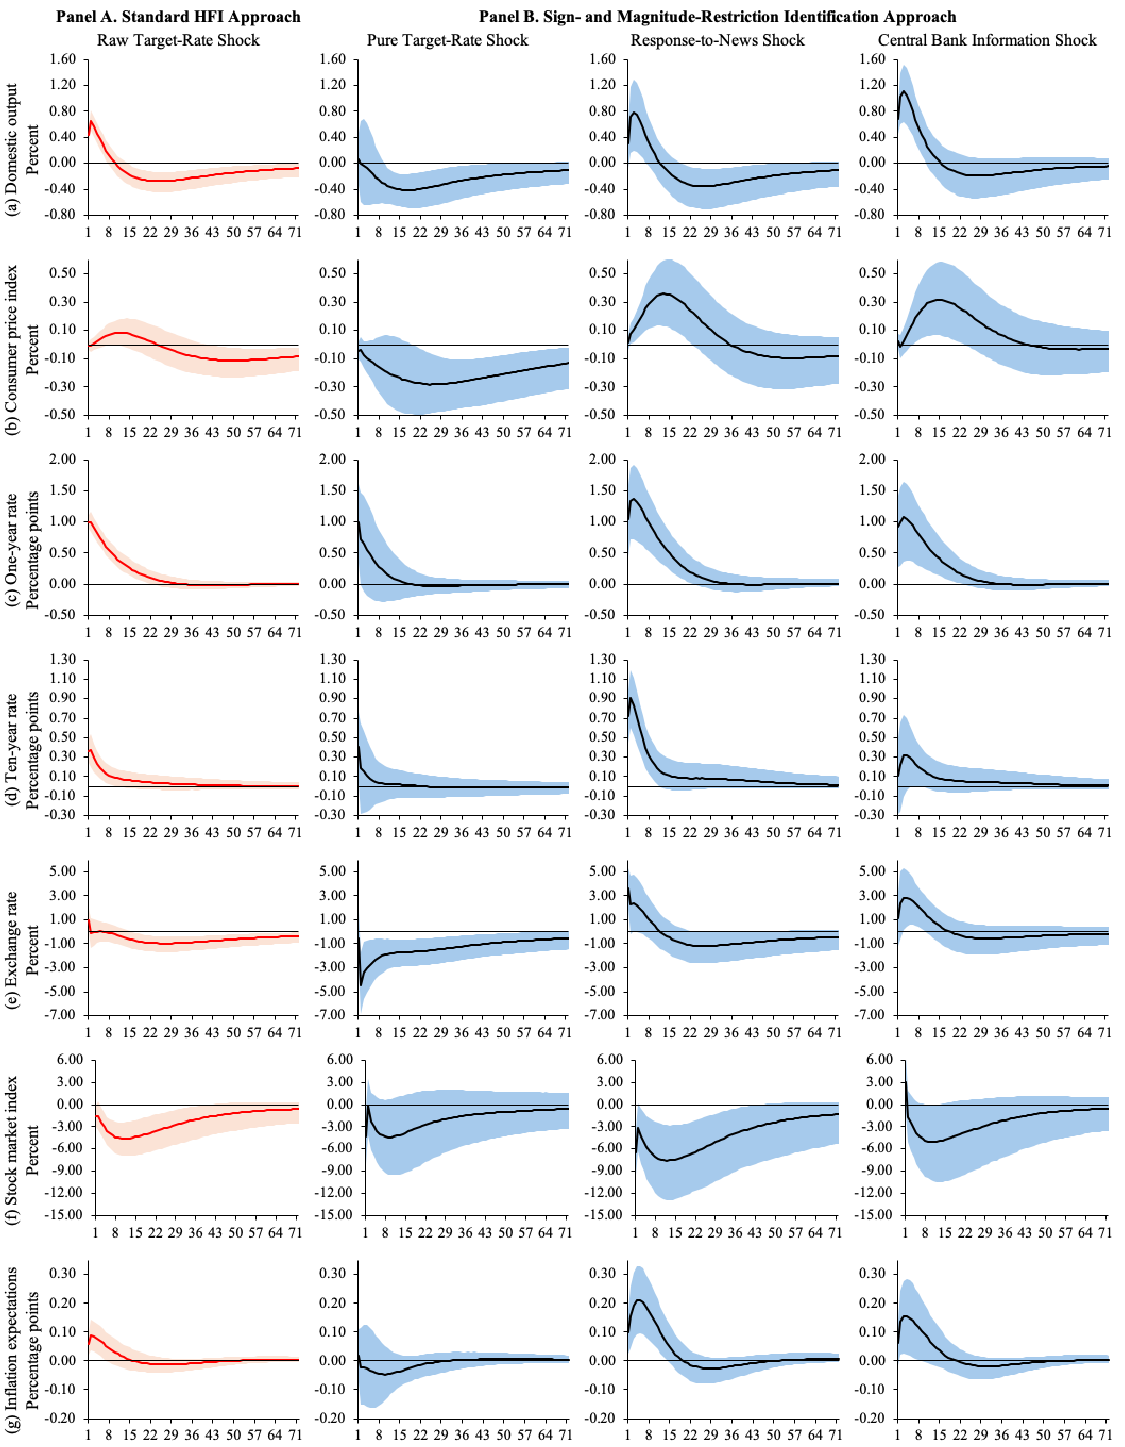
\includegraphics[width=\linewidth]{TR-2024m12-sincerores.pdf}
}
\caption[5pt]{Impulse Responses to Target-Rate, Response-to-News, and Central Bank Information Shocks}
\end{center}
\begin{footnotesize} 
Notes: Responses  are  presented  for a 72-month horizon with the associated 68\% highest posterior density intervals (HPDIs).
\end{footnotesize} 
\end{figure}

\subsection{The Macroeconomic Effects of FG Shocks}

This section analyzes the macroeconomic transmission of news about the \emph{future} path of monetary policy, focusing on FG shocks. While the effects of FG have been extensively studied for AEs, systematic evidence for EMEs remains limited. To the best of our knowledge, this section provides some of the first evidence on the macroeconomic effects of FG shocks in an EME by explicitly disentangling RN and CBI components. As in the previous section, we proceed in two steps. First, we discuss impulse responses obtained under the \emph{standard HFI} specification, which treats the FG surprise as a single MP shock and does not disentangle RN and CBI components. Second, we present results based on the sign- and magnitude-restriction identification, which separately identifies pure FG, RN, and CBI shocks. For comparison, we also reproduce the impulse responses to a contractionary pure target-rate shock reported in \hyperlink{Panel BF1}{Panel~B} of \hyperlink{Figure~1}{Figure~1}. All shocks are normalized to correspond to a one percentage point increase in the one-year rate following an MP shock.

\hyperlink{Panel BF1}{Panel~A} of \hyperlink{Figure~2}{Figure~2} displays, in red, impulse responses to a contractionary FG shock identified under the standard HFI approach, that is, without disentangling RN and CBI components. Impulse responses to a contractionary pure target-rate innovation are reported in green. The plots convey two main messages. First, in contrast to the results for conventional MP shocks presented previously, unpurged FG innovations do not exhibit a clear attenuation bias arising from RN and CBI components. The responses to a contractionary FG shock broadly display the conventional qualitative signs associated with monetary tightening: both the one-year and ten-year yields increase, output contracts, prices decline, equity prices fall, the Mexican peso appreciates, and inflation expectations remain anchored. 

However, compared to the effects of pure target-rate shocks, unpurged FG shocks generate disproportionately large and faster effects on domestic output—a pattern consistent with what has been termed the \emph{forward guidance puzzle} in the literature (see \hyperlink{Del Negro et al. (2023)}{Del Negro et al., 2023}). Output declines by around 0.44\% one month after the shock, exceeding the maximum contraction observed following a target-rate shock, which materializes only after approximately 19 months. These dynamics are difficult to reconcile with the conventional view that monetary policy affects real activity with substantial lags, as well as with the U.S.\ evidence reported by \hyperlink{Swanson (2021, 2024)}{Swanson (2021, 2024)}, who finds that FG shocks generate effects that are comparable to—or even smaller than—those of conventional MP shocks. Moreover, the responses of prices and financial variables—such as the exchange rate and stock prices—also suggest an overstatement of the true effects of FG shocks.

\hyperlink{Panel BF1}{Panel~B} of \hyperlink{Figure~2}{Figure~2} reports impulse responses to the different structural components extracted from FG surprises. As before, we also plot in green the impulse responses to a contractionary pure target-rate shock. Several results emerge from this analysis. First, as shown in the first column, once RN and CBI components are isolated, the contractionary effects of FG shocks become considerably more conservative and closely resemble those of pure target-rate disturbances. This is reflected in the considerable overlap between their impulse responses across macroeconomic and financial variables. Notably, the large and immediate decline in output estimated under the standard HFI approach largely disappears. These findings are more consistent with standard monetary transmission mechanisms and with the recent international evidence reported in \hyperlink{Swanson (2021, 2024)}{Swanson (2021, 2024)}.

Second, in contrast to the results for conventional MP shocks discussed in the previous section, favorable CBI innovations extracted from FG surprises do not systematically exhibit expansionary effects, thereby implying a limited attenuation bias in the estimated effects of FG shocks. One possible interpretation is that the central bank responds to favorable information about economic fundamentals primarily by adjusting the current policy rate, rather than by modifying its communication about the future path of monetary policy.  Consequently, CBI shocks may be more relevant for contaminating target-rate surprises than FG surprises. 

Third, in contrast to hawkish RN shocks identified from target-rate surprises—which are expansionary and tend to attenuate or even reverse the contractionary effects of conventional MP shocks—hawkish RN shocks identified from FG surprises are contractionary and instead distort the estimated effects of FG by amplifying and accelerating their impact. One plausible interpretation is that, following episodes in which economic activity fails to cool as expected, the central bank adopts a more hawkish FG stance to signal a stronger or more persistent commitment to bringing inflation back to target. In such circumstances, RN shocks capture not only the unexpected tightening implied by the policy rule, but also the economy’s ongoing contractionary adjustment already underway. In a VAR that treats raw FG surprises as exogenous shocks, this combination can generate large and immediate contractionary responses, thereby overstating the true effects of FG.


\begin{figure}[htbp]
\hypertarget{Figure 2}{}
\hypertarget{Panel AF2}{}
\hypertarget{Panel BF2}{}
\begin{center}
\resizebox{15cm}{!} {
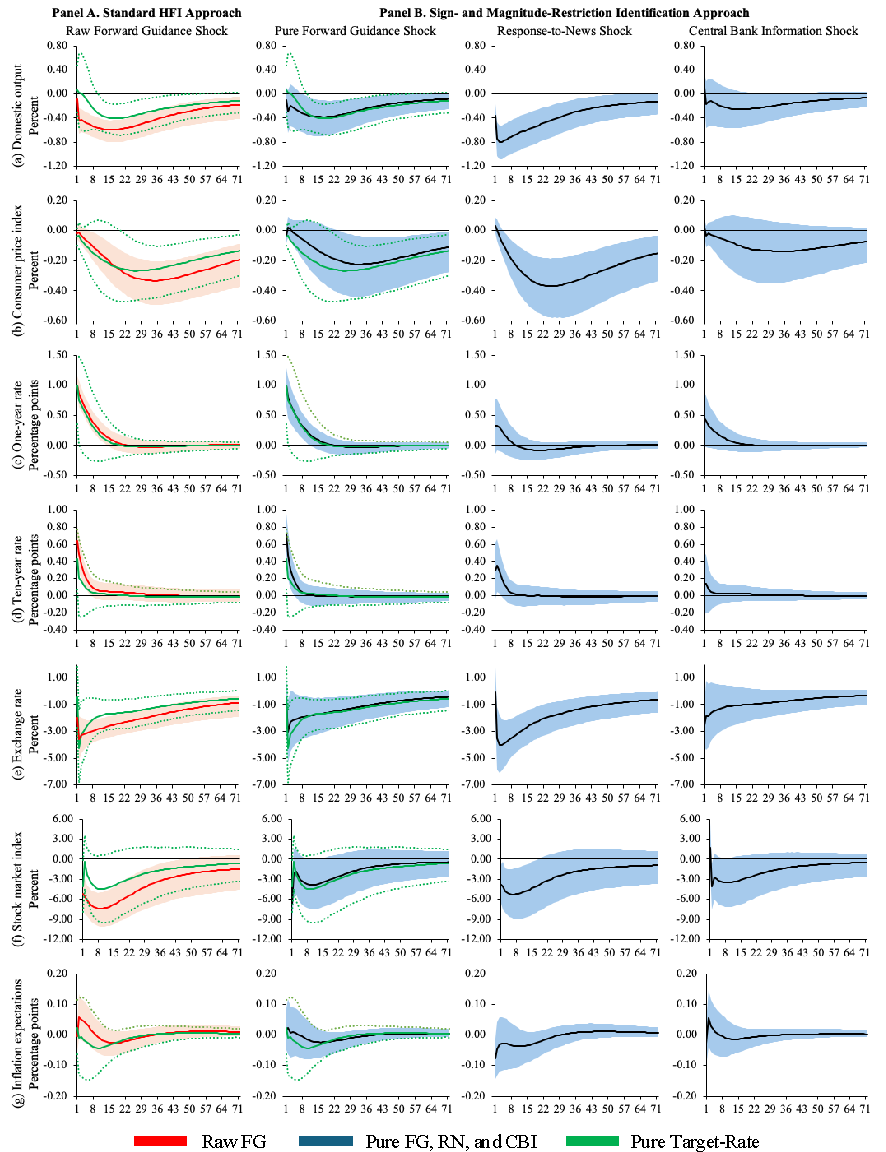
\includegraphics[width=\linewidth]{FG-2024m12_conTR-sincerores.pdf}
}
\caption[5pt]{Impulse Responses to Forward Guidance, Response-to-News, and Central Bank Information Shocks}
\end{center}
\begin{footnotesize} 
Notes: Responses  are  presented  for a 72-month horizon with the associated 68\% highest posterior density intervals (HPDIs).
\end{footnotesize} 
\end{figure}


\subsection{The Importance of Jointly Controlling for RN and CBI}

In this exercise, we compare impulse responses to a contractionary MP shock obtained under four alternative identification strategies. First, the \emph{standard HFI} approach treats the raw monetary policy surprise as a single MP shock and does not separately identify RN or CBI components. Second, the \hyperlink{Jarociński and Karadi (2020)}{Jarociński and Karadi (2020)} approach controls for CBI shocks but does not isolate RN components. Third, the \hyperlink{Bauer and Swanson (2023a, 2023b)}{Bauer and Swanson (2023a, 2023b)} approach controls for RN shocks but does not account for CBI effects. Finally, the \hyperlink{Jarociński and Karadi (2025)}{Jarociński and Karadi (2025)} framework jointly controls for both RN and CBI shocks. All shocks are normalized to correspond to a one percentage point increase in the one-year government bond yield to ensure comparability across specifications.

\hyperlink{Figure 3}{Figure~3} presents the corresponding impulse responses to a contractionary target-rate shock. As can be seen, controlling for only one informational channel, either RN or CBI, helps mitigate the anomalies observed under the standard HFI approach. However, the impulse responses remain attenuated and, in some cases, continue to display counterintuitive dynamics. Only when both RN and CBI components are jointly isolated do the impulse responses become more closely aligned with the predictions of standard macroeconomic models. In this case, output and prices decline more sharply and with shorter delays, the domestic currency appreciates more strongly, and inflation expectations exhibit a clearer negative median response. 

\hyperlink{Figure 4}{Figure~4} presents the corresponding impulse responses to a contractionary FG shock. As documented in the previous section, the main issue with these shocks under the standard HFI approach is that they generate disproportionately large and faster effects—most notably on domestic output. Controlling for CBI shocks alone does not mitigate these anomalies. On the contrary, it appears to amplify them, as evidenced by the stronger responses of output, prices, and the exchange rate. By contrast, controlling for RN shocks substantially attenuates these distortions: the contractionary effects of FG shocks become more moderate and closely resemble those identified under the \hyperlink{Jarociński and Karadi (2025)}{Jarociński and Karadi (2025)} framework. A remaining issue, however, is that inflation expectations exhibit a puzzling increase in response to the contractionary shock when only RN shocks are controlled for. This anomaly is largely resolved once both RN and CBI components are jointly isolated.

Taken together, these results suggest that partial purification of monetary policy surprises may be insufficient. Failing to account simultaneously for both informational channels can lead to biased impulse responses, thereby distorting inference about the true transmission of monetary policy.





\begin{figure}[htbp]
\hypertarget{Figure 2}{}
\hypertarget{Panel AF2}{}
\hypertarget{Panel BF2}{}
\begin{center}
\resizebox{15cm}{!} {
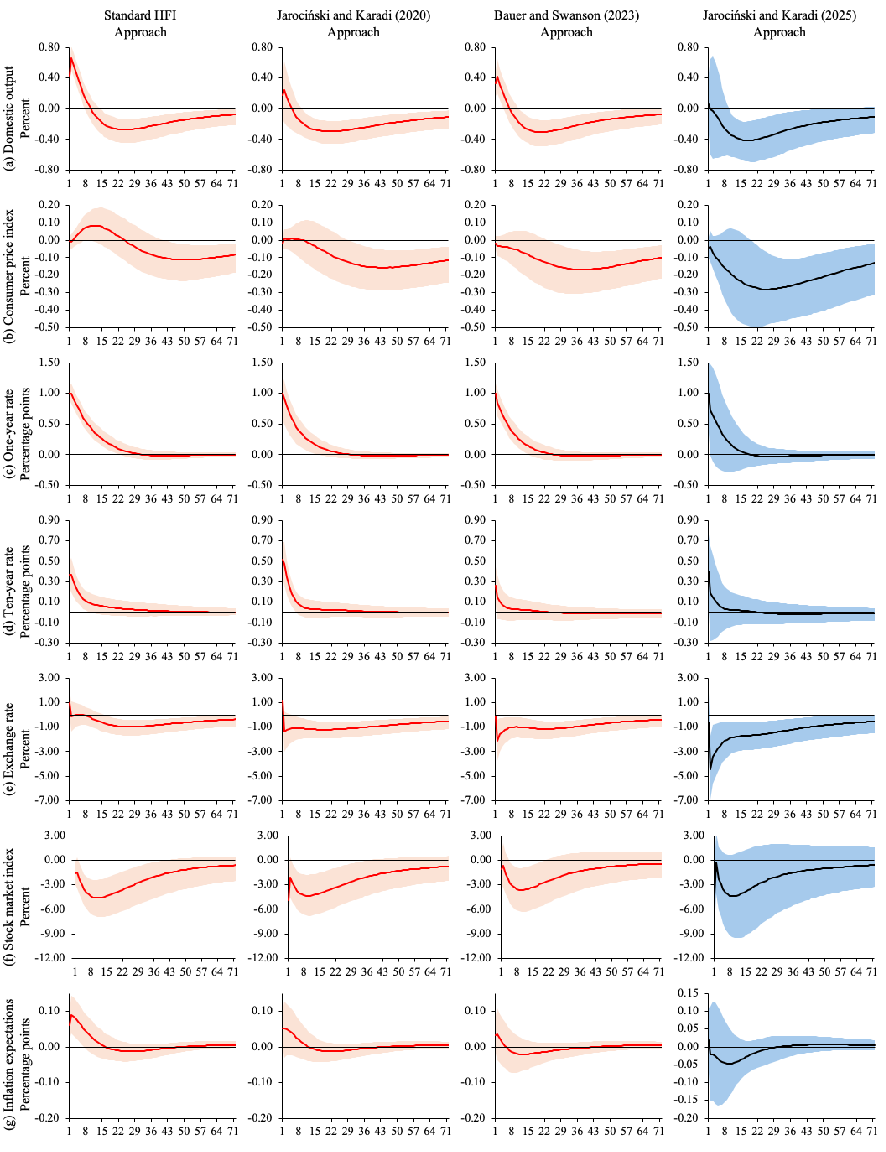
\includegraphics[width=\linewidth]{TR-approaches.pdf}
}
\caption[5pt]{Impulse Responses to Target-Rate Shocks under different Approaches}
\end{center}
\begin{footnotesize} 
Notes: Responses  are  presented  for a 72-month horizon with the associated 68\% highest posterior density intervals (HPDIs).
\end{footnotesize} 
\end{figure}

\begin{figure}[htbp]
\hypertarget{Figure 2}{}
\hypertarget{Panel AF2}{}
\hypertarget{Panel BF2}{}
\begin{center}
\resizebox{15cm}{!} {
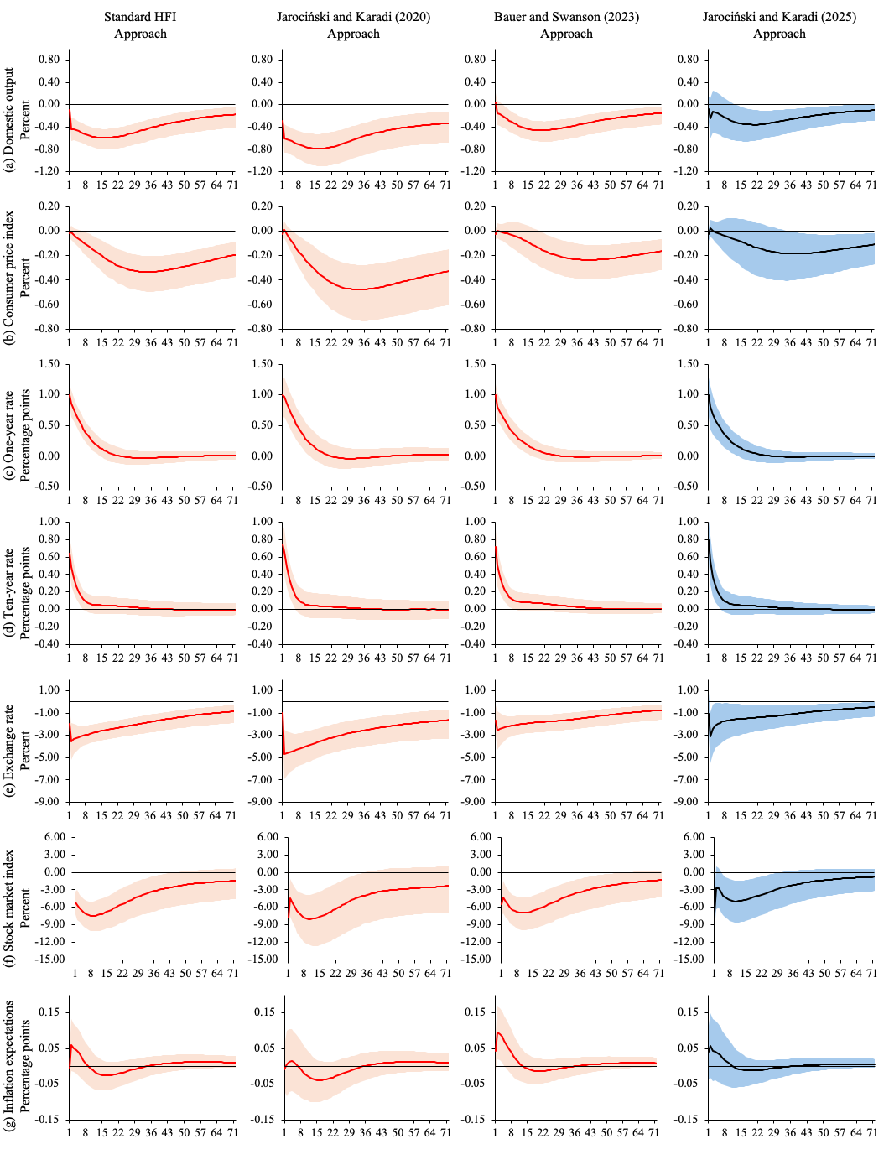
\includegraphics[width=\linewidth]{FG-approaches.pdf}
}
\caption[5pt]{Impulse Responses to Forward Guidance Shocks under different Approaches}
\end{center}
\begin{footnotesize} 
Notes: Responses  are  presented  for a 72-month horizon with the associated 68\% highest posterior density intervals (HPDIs).
\end{footnotesize} 
\end{figure}


\section{Conclusion}
\label{sec:conclusion}

This paper studies the macroeconomic effects of both conventional (target-rate) and unconventional (forward-guidance, FG) monetary policy innovations in Mexico using high-frequency surprises around policy announcements. A central message is that raw interest rate surprises need not be clean measures of exogenous MP shocks: they can embed (i) CBI revealed about fundamentals and (ii) systematic RN components that reflect an imperfectly understood reaction function. When these informational components are not separated, contractionary target-rate shocks exhibit the familiar output, price, and exchange-rate puzzles and are followed by a counterintuitive rise in inflation expectations, while contractionary FG shocks appear to generate disproportionately large and fast real effects.

To address this issue, we combine projections on pre-announcement macro-financial information with high-frequency co-movements in equity prices to disentangle pure monetary policy innovations from RN and CBI shocks. Once CBI and RN components are isolated, the estimated effects of contractionary target-rate shocks become broadly consistent with standard transmission mechanisms, featuring delayed contractions in output and prices, an appreciation of the domestic currency, and well-anchored inflation expectations. For FG, isolating RN shocks substantially attenuates the apparent “forward guidance puzzle”: the implied macroeconomic effects become more conservative and broadly similar to those of pure target-rate shocks.

A key contribution is that RN components play \emph{asymmetric} contamination roles across policy instruments. In our estimates, RN shocks embedded in target-rate surprises tend to attenuate the contractionary effects of conventional MP shocks, while RN shocks embedded in FG surprises instead amplify and accelerate the effects of FG innovations. Beyond distinguishing conventional from unconventional tools, the results also speak to the exchange-rate puzzle in EMEs by highlighting how omitted informational components can distort estimated exchange-rate responses to policy tightenings.

Overall, the findings underscore that credible measurement of MP shocks in EMEs requires explicitly accounting for informational and systematic policy-response components in high-frequency surprises. Doing so yields impulse responses that are more interpretable, more comparable across policy tools, and more consistent with conventional monetary transmission.



\newpage

\begin{thebibliography}{99}

\bibitem{} \hypertarget{Aleem (2010)}{} 
Aleem, A. (2010). Transmission mechanism of monetary policy in India. \textit{Journal of Asian Economics} \textbf{21}(2), 186-197.

\bibitem{} \hypertarget{Andrade and Ferroni (2021)}{} Andrade, P., and Ferroni, F. (2021). Delphic and odyssean monetary policy shocks: Evidence from the euro area. \textit{Journal of Monetary Economics} \textbf{117}, 816-832.

\bibitem{} \hypertarget{Angeles et al. (2019)}{}
Angeles Galván, D., Cortés Espada, J. F., and Sámano, D. (2019). Evolución y características del traspaso del tipo de cambio a precios en México. (No. 2019-10). Banco de México Working Paper.

\bibitem{} \hypertarget{Andersen et al. (2003)}{} 
Andersen, T. G., Bollerslev, T., Diebold, F. X., and Vega, C. (2003). Micro effects of macro announcements: Real-time price discovery in foreign exchange. \textit{American economic review} \textbf{93}(1), 38-62.

\bibitem{} \hypertarget{Andersen et al. (2007)}{} 
Andersen, T. G., Bollerslev, T., Diebold, F. X., and Vega, C. (2007). Real-time price discovery in global stock, bond and foreign exchange markets. \textit{Journal of international Economics} \textbf{73}(2), 251-277.

\bibitem{} \hypertarget{Banco de Mexico (2008)}{} Banco de México (2008). Annual inflation report.

\bibitem{} \hypertarget{Bancoa}{} Banco de México (2021). Quarterly inflation report. April-June.

\bibitem{} \hypertarget{Barakchian and Crowe (2013)}{} 
Barakchian, S. M., and Crowe, C. (2013). Monetary policy matters: Evidence from new shocks data. \textit{Journal of Monetary Economics} \textbf{60}(8), 950-966.

\bibitem{} \hypertarget{Bauer and Rudebusch (2016)}{} 
Bauer, M. D., and Rudebusch, G. D. (2016). Monetary policy expectations at the zero lower bound. \textit{Journal of Money, Credit and Banking}, \textbf{48}(7), 1439-1465.

\bibitem{} \hypertarget{Bauer and Swanson (2023a)}{} 
Bauer, M. D., and Swanson, E. T. (2023a). An alternative explanation for the ``fed information effect''. \textit{American Economic Review} \textbf{113}(3), 664-700.

\bibitem{} \hypertarget{Bauer and Swanson (2023b)}{} 
Bauer, M. D., and Swanson, E. T. (2023b). A reassessment of monetary policy surprises and high-frequency identification. \textit{NBER Macroeconomics Annual} \textbf{37}(1), 87-155.

\bibitem{} \hypertarget{Bernanke and Blinder (1992)}{}Bernanke, B. S., \& Blinder, A. S. (1992). The Federal Funds Rate and the Channels of Monetary Transmission. \textit{American Economic Review}, \textbf{82}(4), 901–921.

\bibitem{} \hypertarget{Bernanke and Gertler (1995)}{}Bernanke, B. S., \& Gertler, M. (1995). Inside the Black Box: The Credit Channel of Monetary Policy Transmission. \textit{Journal of Economic Perspectives}, \textbf{9}(4), 27–48.

\bibitem{} \hypertarget{Bernanke and Kuttner (2005)}{} 
Bernanke, B. S., and Kuttner, K. N. (2005). What explains the stock market's reaction to Federal Reserve policy? \textit{The Journal of Finance} \textbf{60}(3), 1221-1257.

\bibitem{} \hypertarget{Bjørnland (2009)}{}Bjørnland, H. C. (2009). Monetary policy and exchange rate overshooting: Dornbusch was right after all. \textit{Journal of International Economics} \textbf{79}(1), 64-77.

\bibitem{} \hypertarget{Blinder et al. (2008)}{}Blinder, A. S., Ehrmann, M., Fratzscher, M., De Haan, J., and Jansen, D. J. (2008). Central bank communication and monetary policy: A survey of theory and evidence. \textit{Journal of Economic Literature} \textbf{46}(4), 910-945.

\bibitem{} \hypertarget{Boivin, et al. (2010)}{}Boivin, J., Kiley, M. T., and Mishkin, F. S. (2010). How has the monetary transmission mechanism evolved over time? \textit{Handbook of monetary economics} \textbf{3}, 369-422.

\bibitem{} \hypertarget{Bredin et al. (2010)}{}Bredin, D., Hyde, S., and Reilly, G. O. (2010). Monetary policy surprises and international bond markets. \textit{Journal of International Money and Finance} \textbf{29}(6), 988-1002.

\bibitem{} \hypertarget{Caldara and Herbst (2019)}{} Caldara, D., and Herbst, E. (2019). Monetary policy, real activity, and credit spreads: Evidence from Bayesian proxy SVARs. \textit{American Economic Journal: Macroeconomics} \textbf{11}(1), 157-92.

\bibitem{} \hypertarget{Campbell et al. (2012)}{} Campbell, J. R., Evans, C. L., Fisher, J. D., Justiniano, A., Calomiris, C. W., and Woodford, M. (2012). Macroeconomic effects of federal reserve forward guidance. \textit{Brookings Papers on Economic Activity} \textbf{42}(1), 1-80.

\bibitem{} \hypertarget{Canova and De Nicolo (2002)}{}Canova, F., and De Nicolo, G. (2002). Monetary disturbances matter for business fluctuations in the G-7. \textit{Journal of Monetary Economics} \textbf{49}(6), 49(6), 1131-1159.

\bibitem{} \hypertarget{Capistrán et al. (2012)}{}Capistrán, C., Ibarra, R., and Ramos Francia, M. (2012). El traspaso de movimientos del tipo de cambio a los precios. Un análisis para la economía mexicana. \textit{El Trimestre Económico} \textbf{79}(316), 813-838.

\bibitem{} \hypertarget{Capistran at al. (2019)}{}Capistrán, C., Chiquiar, D., and Hernández, J. R. (2019). Identifying Dornbusch's exchange rate overshooting with structural VECs: evidence from Mexico. \textit{61st issue (December 2019) of the International Journal of Central Banking}.

\bibitem{} \hypertarget{Carrillo and Elizondo (2015)}{}Carrillo, J. A., and Elizondo, R. (2015). How robust are SVARs at measuring monetary policy in small open economies? (No. 2015-18). Banco de México Working Paper.

\bibitem{} \hypertarget{Carrillo et al. (2020)}{} Carrillo, J. A., Elizondo, R., and Hernández-Román, L. G. (2020). Inquiry on the transmission of US aggregate shocks to Mexico: a SVAR approach. \textit{Journal of International Money and Finance} \textbf{104}, 1-24.

\bibitem{} \hypertarget{Carrillo et al. (2025)}{}Carrillo, J., Elizondo, R., Hernández-Román, L., Ibarra, R., and Quiroga, M. (2025). Monetary policy transmission in a small open economy
before and after the pandemic: the case of Mexico. Banco de México, mimeo.

\bibitem{} \hypertarget{Cesa-Bianchi et al. (2020)}{}
Cesa-Bianchi, A., Thwaites, G., and Vicondoa, A. (2020). Monetary policy transmission in the United Kingdom: A high frequency identification approach. \textit{European Economic Review} \textbf{123}, 103375.

\bibitem{} \hypertarget{Cesa (2022)}{} Cesa-Bianchi, A., and Sokol, A. (2022). Financial shocks, credit spreads, and the international credit channel. \textit{Journal of International Economics} \textbf{135}, 1-18.

\bibitem{} \hypertarget{Cespedes et al. (2008)}{} 
Céspedes, B., Lima, E., and Maka, A. (2008). Monetary policy, inflation and the level of economic activity in Brazil after the real plan: stylized facts from SVAR models. \textit{Revista Brasileira de Economia} \textbf{62}, 123-160.

\bibitem{} \hypertarget{Checo et al. (2024)}{}Checo, A., Grigoli, F., and Sandri, D. (2024). Monetary policy transmission in emerging markets: proverbial concerns, novel evidence (No. 1170). Bank for International Settlements Working Papers.

\bibitem{} \hypertarget{Chiguil-Rojas et al. (2024)}{} 
Chiguil-Rojas, A., Esquivel, G., and Leal, J. (2024). La transmisión de la política monetaria a través del crédito bancario en México. \textit{El Trimestre Económico} \textbf{91}(363), 603-662.

\bibitem{} \hypertarget{Christiano et al. (2005)}{}Christiano, L. J., Eichenbaum, M., and Evans, C. L. (2005). Nominal rigidities and the dynamic effects of a shock to monetary policy. \textit{Journal of Political Economy} \textbf{113}(1), 1-45.

\bibitem{} \hypertarget{Colunga (2020)}{} 
Colunga, L. F. (2020). The loan puzzle in México. \textit{Working Papers}.

\bibitem{} \hypertarget{Copelman and Werner (1997)}{} 
Copelman, M., and Werner, A. M. (1997). El mecanismo de la transmisión monetaria en México. \textit{El Trimestre Económico} \textbf{64}(253), 75-104.

\bibitem{} \hypertarget{Cortés (2013)}{}Cortés, J. F. (2013). Estimación del traspaso del tipo de cambio a los precios en México. \textit{Monetaria} \textbf{35}(2), 312-4344.

\bibitem{} \hypertarget{Cuadra (2008)}{}Cuadra, G. (2008). Hechos estilizados del ciclo económico en México. \textit{Banco de México, Documentos de Investigación} \textbf{2008-14}.

\bibitem{} \hypertarget{Cushman and Zha (1997)}{}Cushman, D. O., and Zha, T. (1997). Identifying monetary policy in a small open economy under flexible exchange rates. \textit{Journal of Monetary Economics} \textbf{39}(3), 433-448.

\bibitem{} \hypertarget{Deb et al. (2023)}{}Deb, M. P., Estefania-Flores, J., Firat, M., Furceri, D., and Kothari, S. (2023). Monetary policy transmission heterogeneity: cross-country evidence (WP/23/204). International Monetary Fund Working Papers.

\bibitem{} \hypertarget{Degasperi et al. (2023)}{}
Degasperi, R., Hong, S. S., and Ricco, G. (2023). The global transmission of U.S. monetary policy. CREST Working Paper 2023-02.

\bibitem{} \hypertarget{Diaz de Leon and Greenham (2001)}{} 
Díaz de León, A., and Greenham, L. (2001). Política monetaria y tasas de interés: experiencia reciente para el caso de México. \textit{Economía Mexicana Nueva Época} \textbf{10}(2), 213-258.

\bibitem{} \hypertarget{Disyatat and Vongsinsirikul (2003)}{}Disyatat, P., and Vongsinsirikul, P. (2003). Monetary policy and the transmission mechanism in Thailand. \textit{Journal of Asian Economics} \textbf{14}(3), 389-418.

\bibitem{} \hypertarget{Dornbusch (1976)}{}Dornbusch, R. (1976). Expectations and exchange rate dynamics. \textit{Journal of Political Economy} \textbf{84}(6), 1161-1176.

\bibitem{} \hypertarget{Ehrmann and Fratzscher (2003)}{}Ehrmann, M., and Fratzscher, M. (2003). Monetary policy announcements and money markets: A transatlantic perspective. \textit{International Finance} \textbf{6}(3), 309-328.

\bibitem{} \hypertarget{Ehrmann and Fratzscher (2005)}{}Ehrmann, M., and Fratzscher, M. (2005). Equal size, equal role? Interest rate interdependence between the euro area and the United States. \textit{The Economic Journal} \textbf{115}(506), 928-948.

\bibitem{} \hypertarget{Eichenbaum and Evans (1995)}{}Eichenbaum, M., and Evans, C. L. (1995). Some empirical evidence on the effects of shocks to monetary policy on exchange rates. \textit{The Quarterly Journal of Economics} \textbf{110}(4), 975-1009.

\bibitem{} \hypertarget{Elizondo (2012)}{}Elizondo, R. (2012). Estimaciones del PIB mensual basadas en el IGAE (No. 2012-11). Banco de México Working Paper.

\bibitem{} \hypertarget{Faust et al. (2007)}{}Faust, J., Rogers, J. H., Wang, S. Y. B., and Wright, J. H. (2007). The high-frequency response of exchange rates and interest rates to macroeconomic announcements. \textit{Journal of Monetary Economics} \textbf{54}(4), 1051-1068.

\bibitem{} \hypertarget{Favara (2016)}{} Favara, G., Gilchrist, S., Lewis, K. F., and Zakrajsek, E. (2016). Recession risk and the excess bond premium. (No. 2016-04-08). Board of Governors of the Federal Reserve System (US).

\bibitem{} \hypertarget{Ferrari et al. (2021)}{}Ferrari, M., Kearns, J., and Schrimpf, A. (2021). Monetary policy’s rising FX impact in the era of ultra-low rates. \textit{Journal of Banking \& Finance} \textbf{129}, 1-13.

\bibitem{} \hypertarget{Fink (2015)}{} Fink, F., and Schüler, Y. S. (2015). The transmission of US systemic financial stress: Evidence for emerging market economies. \textit{Journal of International Money and Finance} \textbf{55}, 6-26.

\bibitem{} \hypertarget{Friedman (1961)}{} Friedman, M. (1961). The lag in effect of monetary policy. \textit{Journal of Political Economy} \textbf{69}(5), 447-466.

\bibitem{} \hypertarget{Gali and Monacelli (2005)}{} Galí, J., and Monacelli, T. (2005). Monetary policy and exchange rate volatility in a small open economy. \textit{Review of Economic Studies} \textbf{72}(3), 707–734.

\bibitem{} \hypertarget{Garcés (2001)}{}Garcés, D. (2001). Determinación del nivel de precios y la dinámica inflacionaria en México. \textit{Monetaria} \textbf{24}(3), 241-269.

\bibitem{} \hypertarget{Garcia (2007)}{}Gaytán, A., and González García, J. R. (2007). Cambios estructurales en el mecanismo de transmisión de la política monetaria en México: un enfoque VAR no lineal. \textit{Monetaria} \textbf{30}(4), 367-404.

\bibitem{} \hypertarget{Gaytan and Gonzalez-Garcia (2007)}{}
Gaytán, A., and González-García, J. (2007). Cambios estructurales en el mecanismo de transmisión de la política monetaria en México: Un enfoque VAR no lineal. \textit{Monetaria} \textbf{30}(4), 367-404.

\bibitem{} \hypertarget{Gertler and Karadi (2015)}{}Gertler, M., and Karadi, P. (2015). Monetary policy surprises, credit costs, and economic activity. \textit{American Economic Journal: Macroeconomics} \textbf{7}(1), 44-76.

\bibitem{} \hypertarget{Gilchrist (2012)}{}Gilchrist, S., and Zakrajšek, E. (2012). Credit spreads and business cycle fluctuations. \textit{American Economic Review} \textbf{102}(4), 1692-1720.

\bibitem{} \hypertarget{Grilli and Roubini (1995)}{} Grilli, V., and Roubini, N. (1995). Liquidity and exchange rates: puzzling evidence from the G-7 countries (No. 95-17). Stern School of Business Working Paper.

\bibitem{} \hypertarget{Gurkaynak et al. (2005)}{} Gürkaynak, R. S., Sack, B., and Swanson, E. T. (2005). Do actions speak louder than words? The response of asset prices to monetary policy actions and statements. \textit{International Journal of Central Banking} \textbf{1}(1), 55-93.

\bibitem{} \hypertarget{Ha and So (2023)}{}Ha, J., and So, I. (2023). Which monetary shocks matter in small open economies? Evidence from Canada. \textit{International Journal of Central Banking} \textbf{19}(2), 389-472.

\bibitem{} \hypertarget{Hanson and Stein (2015)}{}
Hanson, S. G., and Stein, J. C. (2015). Monetary policy and long-term real rates. \textit{Journal of Financial Economics} \textbf{115}(3), 429-448.

\bibitem{} \hypertarget{Hausman and Wongswan (2011)}{}Hausman, J., and Wongswan, J. (2011). Global asset prices and FOMC announcements. \textit{Journal of International Money and Finance} \textbf{30}(3), 547-571.

\bibitem{} \hypertarget{Havranek and Rusnak (2018)}{} Havranek, T., and Rusnak, M. (2018). Transmission lags of monetary policy: A meta-analysis. \textit{33rd issue (December 2013) of the International Journal of Central Banking}.

\bibitem{} \hypertarget{Iacoviello and Navarro (2019)}{} Iacoviello, M., and Navarro, G. (2019). Foreign effects of higher US interest rates. \textit{Journal of International Money and Finance} \textbf{95}, 232-250.

\bibitem{} \hypertarget{Ibarra (2016)}{}Ibarra, R. (2016). How important is the credit channel in the transmission of monetary policy in Mexico? \textit{Applied Economics} \textbf{48}(36), 3462-3484.

\bibitem{} \hypertarget{Ibarra (2023)}{}
Ibarra, R. (2023). The Yield Spread as a Predictor of Economic Activity in Mexico: The Role of the Term Premium. \textit{Economía LACEA Journal} \textbf{22}(1), 153–174.

\bibitem{} \hypertarget{Jaramillo et al. (2019)}{}Jaramillo, J., Pech Moreno, L. A., Ramírez, C., and Sanchez-Amador, D. (2019). Nonlinear exchange rate pass-through in Mexico. (No. 2019-16). Banco de México Working Paper.

\bibitem{} \hypertarget{JK (2020)}{} Jarociński, M., and Karadi, P. (2020). Deconstructing monetary policy surprises—the role of information shocks. \textit{American Economic Journal: Macroeconomics} \textbf{12}(2), 1-43.

\bibitem{} \hypertarget{Jentsch and Lunsford (2019)}{}
Jentsch, C., and Lunsford, K. G. (2019). Inference in structural vector autoregressions identified with external instruments. \textit{Journal of the American Statistical Association} \textbf{114}(528), 1638–1650.

\bibitem{} \hypertarget{Jentsch and Lunsford (2019b)}{} 
Jentsch, C., and Lunsford, K. G. (2019). The dynamic effects of personal and corporate income tax changes in the United States: Comment. \textit{American Economic Review} \textbf{109}(7), 2655-2678.

\bibitem{} \hypertarget{Jorda (2009)}{}
Jordà, Ò. (2009). Simultaneous confidence regions for impulse responses. \textit{The Review of Economics and Statistics} \textbf{91}(3), 629–647.

\bibitem{} \hypertarget{Kerssenfischer (2022)}{} Kerssenfischer, M. (2022). Information effects of euro area monetary policy. \textit{Economics Letters} \textbf{216}, 1-5.

\bibitem{} \hypertarget{Kim and Singleton (2012)}{} Kim, D. H., and Singleton, K. J. (2012). Term structure models and the zero bound: an empirical investigation of Japanese yields. \textit{Journal of Econometrics}, \textbf{170}(1), 32-49.

\bibitem{} \hypertarget{Kim and Lim (2022)}{}Kim, S., and Lim, K. (2022). Effects of monetary policy shocks on exchange rate in emerging countries. \textit{The World Economy} \textbf{45}(4), 1242-1261.

\bibitem{} \hypertarget{Kim et al. (2017)}{}Kim, S. H., Moon, S., and Velasco, C. (2017). Delayed overshooting: Is it an’80s puzzle? \textit{Journal of Political Economy} \textbf{125}(5), 1570-1598.

\bibitem{} \hypertarget{Kochen and Sámano (2016)}{} 
Kochen, F., and Sámano, D. (2016). Price-setting and exchange rate pass-through in the Mexican economy: Evidence from CPI micro data. (No. 2016-13). Banco de México Working Paper.

\bibitem{} \hypertarget{Krippner (2013)}{} Krippner, L. (2013). Measuring the stance of monetary policy in zero lower bound environments. \textit{Economics Letters}, \textbf{118}(1), 135-138.

\bibitem{} \hypertarget{Kuttner (2001)}{} Kuttner, K. N. (2001). Monetary policy surprises and interest rates: Evidence from the Fed funds futures market. \textit{Journal of Monetary Economics} \textbf{47}(3), 523-544.

\bibitem{} \hypertarget{Linde (2003)}{}Lindé, J. (2003). Monetary policy shocks and business cycle fluctuations in a small open economy: Sweden 1986-2002 (No. 153). Sveriges Riksbank Working Paper Series.

\bibitem{} \hypertarget{Lombardi et al. (2018)}{}
Lombardi, D., Siklos, P., and St. Amand, S. (2018). A survey of the international evidence and lessons learned about unconventional monetary policies: Is a ‘new normal’in our future? \textit{Journal of Economic Surveys} \textbf{32}(5), 1229-1256.

\bibitem{} \hypertarget{Mackowiak (2007)}{} Maćkowiak, B. (2007). External shocks, US monetary policy and macroeconomic fluctuations in emerging markets. \textit{Journal of Monetary Economics} \textbf{54}(8), 2512-2520.

\bibitem{} \hypertarget{Mankiw (2009)}{}
Mankiw, N. G. (2009). \textit{Macroeconomics}. 7th Edition. Worth Publishers, New York.

\bibitem{} \hypertarget{Mallick and Sousa (2012)}{} 
Mallick, S. K., and Sousa, R. M. (2012). Real effects of monetary policy in large emerging economies. \textit{Macroeconomic Dynamics} \textbf{16}(S2), 190-212.

\bibitem{} \hypertarget{Martinez et al. (2001)}{}Martínez, L., Sánchez, O., and Werner, A. (2001). Consideraciones sobre la conducción de la política monetaria y el mecanismo de transmisión en México (No. 2001-02). Banco de México Working Paper.

\bibitem{} \hypertarget{Melosi (2017)}{} Melosi, L. (2017). Signalling effects of monetary policy. \textit{The Review of Economic Studies} \textbf{84}(2), 853-884.

\bibitem{} \hypertarget{Mertens and Ravn (2013)}{}Mertens, K., and Ravn, M. O. (2013). The dynamic effects of personal and corporate income tax changes in the United States. \textit{American economic review} \textbf{103}(4), 1212-1247.

\bibitem{} \hypertarget{Mertens and Ravn (2019)}{}
Mertens, K., and Ravn, M. O. (2019). The dynamic effects of personal and corporate income tax changes in the United States: Reply. \textit{American Economic Review} \textbf{109}(7), 2679–2691.

\bibitem{} \hypertarget{Minella (2003)}{} 
Minella, A. (2003). Monetary policy and inflation in Brazil (1975-2000): a VAR estimation. \textit{Revista Brasileira de Economia} \textbf{57}, 605-635.

\bibitem{} \hypertarget{Miranda-Agrippino and Ricco (2021)}{} 
Miranda-Agrippino, S., and Ricco, G. (2021). The transmission of monetary policy shocks. \textit{American Economic Journal: Macroeconomics} \textbf{13}(3), 74-107.

\bibitem{} \hypertarget{Mishkin (1995)}{}Mishkin, F. S. (1995). Symposium on the monetary transmission mechanism. \textit{Journal of Economic perspectives} \textbf{9}(4), 3-10.

\bibitem{} \hypertarget{Moessner et al. (2017)}{} Moessner, R., Jansen, D.-J., and de Hann, J. (2017). Communication about future policy rates in 
theory and practice: a survey. \textit{Journal of Economic Surveys} \textbf{31}(3), 678-711.

\bibitem{} \hypertarget{Morsink and Bayoumi (2001)}{} Morsink, J., and Bayoumi, T. (2001). A peek inside the black box: the monetary transmission mechanism in Japan. \textit{IMF Staff Papers} \textbf{48}(1), 22-57.

\bibitem{} \hypertarget{Murno (2025)}{}
Murno, J. (2025). EMTA Survey: Second Quarter 2025 Emerging Markets Debt Trading at US\$1.464 Trillion. Emerging Markets Traders Association, Press Release, September 29, 2025.

\bibitem{} \hypertarget{Nakamura and Steinsson (2018)}{} 
Nakamura, E., and Steinsson, J. (2018). High-frequency identification of monetary non-neutrality: the information effect. \textit{The Quarterly Journal of Economics} \textbf{133}(3), 1283-1330.

\bibitem{} \hypertarget{Nguyen (2020)}{}Nguyen, T. M. L. (2020). Output effects of monetary policy in emerging and developing countries: Evidence from a meta-analysis. \textit{Emerging Markets Finance and Trade} \textbf{56}(1), 68-85.

\bibitem{} \hypertarget{Ormaechea and Fernandez (2011)}{} 
Ormaechea, M. S. A., and Fernandez, M. D. C. (2011). The monetary transmission in dollarized and non-dollarized economies: the cases of Chile, New Zealand, Peru and Uruguay. \textit{International Monetary Fund}.

\bibitem{} \hypertarget{Otero (2015)}{}
Otero, J. D. Q. (2015). Impactos de la política monetaria y canales de transmisión en países de América Latina con esquema de inflación objetivo. \textit{Ensayos sobre Política Económica} \textbf{33}(76), 61–75.

\bibitem{} \hypertarget{Orphanides (2001)}{}Orphanides, A. (2001). Monetary Policy Rules Based on Real-Time Data. \textit{American Economic Review}, \textbf{91}(4), 964–985.

\bibitem{} \hypertarget{Racette and Raynauld (1992)}{}Racette, D., and Raynauld, J. (1992). Canadian monetary policy: will the checklist approach ever get us to price stability? \textit{Canadian Journal of Economics}, 819-838.

\bibitem{} \hypertarget{Ramey (1993)}{}
Ramey, V. A. (1993). How important is the credit channel in the transmission of monetary policy? \textit{Carnegie-Rochester Conference Series on Public Policy} \textbf{39}(1), 1-45.

\bibitem{} \hypertarget{Ramos-Francia and Torres (2008)}{} 
Ramos-Francia, M., and Torres, A. (2008). Inflation dynamics in Mexico: a characterization using the new Phillips curve. \textit{The North American Journal of Economics and Finance} \textbf{19}(3), 274-289.

\bibitem{} \hypertarget{Rogers et al. (2014)}{}Rogers, J. H., Scotti, C., and Wright, J. H. (2014). Evaluating asset-market effects of unconventional monetary policy: a multi-country review. \textit{Economic Policy} \textbf{29}(80), 749-799.

\bibitem{} \hypertarget{Romer and Romer (2000)}{} 
Romer, C. D., and Romer, D. H. (2000). Federal Reserve information and the behavior of interest rates. \textit{American Economic Review} \textbf{90}(3), 429-457.

\bibitem{} \hypertarget{Romer and Romer (2004)}{}Romer, C. D., and Romer, D. H. (2004). A new measure of monetary shocks: Derivation and implications. \textit{American Economic Review} \textbf{94}(4), 1055-1084.

\bibitem{} \hypertarget{Rosa (2011)}{}Rosa, C. (2011). The high-frequency response of exchange rates to monetary policy actions and statements. \textit{Journal of Banking \& Finance} \textbf{35}(2), 35(2), 478-489.

\bibitem{} \hypertarget{Rusnak et al. (2013)}{} Rusnák, M., Havranek, T., and Horváth, R. (2013). How to solve the price puzzle? A meta‐analysis. \textit{Journal of Money, Credit and Banking} \textbf{45}(1), 37-70.

\bibitem{}  \hypertarget{Sidaoui and Ramos-Francia (2008)}{}Sidaoui, J. and Ramos-Francia, M. (2008). The monetary transmission mechanism in Mexico: recent developments. BIS Papers, \textbf{35}, 363-394.

\bibitem{} \hypertarget{Sims (1980)}{}Sims, C. A. (1980). Macroeconomics and reality. \textit{Econometrica: Journal of the Econometric Society} \textbf{48}, 1-48.

\bibitem{} \hypertarget{Sims (1992)}{}Sims, C. A. (1992). Interpreting the macroeconomic time series facts: The effects of monetary policy. \textit{European Economic Review} \textbf{36}(5), 975-1000.

\bibitem{} \hypertarget{Sims et al. (1990)}{}Sims, C. A., Stock, J. H., \& Watson, M. W. (1990). Inference in Linear Time Series Models with Some Unit Roots. \textit{Econometrica}, \textbf{58}(1), 113–144.

\bibitem{} \hypertarget{Sims and Zha (2006)}{}Sims, C. A., and Zha, T. (2006). Does monetary policy generate recessions? \textit{Macroeconomic Dynamics} \textbf{10}(2), 231-272.

\bibitem{} \hypertarget{Solis (2023a)}{}Solís, P. (2023a). Does the exchange rate respond to monetary policy in Mexico? Solving an exchange rate puzzle in emerging markets. \textit{Journal of Money, Credit and Banking} \textbf{55}(8), 2093-2113.

\bibitem{} \hypertarget{Solis (2023b)}{}Solís, P. (2023b). Do central bank words matter in emerging markets? Evidence from Mexico. \textit{Journal of Macroeconomics} \textbf{78}, 1-16.

\bibitem{} \hypertarget{Soosalu (2024)}{} 
Soosalu, M. (2024). Monetary policy transmission in Canada - A high frequency identification approach. \textit{The B.E. Journal of Macroeconomics} \textbf{24}(2), 781-811.

\bibitem{} \hypertarget{Stock and Watson (2002)}{}Stock, J. H., and Watson, M. W. (2002). Macroeconomic forecasting using diffusion indexes. \textit{Journal of Business \& Economic Statistics} \textbf{}\textbf{20}(2), 147-162.

\bibitem{} \hypertarget{Stock and Watson (2012)}{}Stock, J. H., and Watson, M. W. (2012). Disentangling the Channels of the 2007-09 Recession. \textit{Brookings Papers on Economic Activity} \textbf{}\textbf{42}(1), 81-135.

\bibitem{} \hypertarget{Stock and Watson (2018)}{}Stock, J. H., and Watson, M. W. (2018). Identification and estimation of dynamic causal effects in macroeconomics using external instruments. \textit{The Economic Journal} \textbf{128}(610), 917-948.

\bibitem{} \hypertarget{Stock et al. (2002)}{}Stock, J. H., Wright, J. H., and Yogo, M. (2002). A survey of weak instruments and weak identification in generalized method of moments. \textit{Journal of Business and Economic Statistics} \textbf{20}(4), 518-529. 

\bibitem{} \hypertarget{Swanson and Williams (2014)}{} Swanson, E. T., and Williams, J. C. (2014). Measuring the effect of the zero lower bound on medium-and longer-term interest rates. \textit{American Economic Review} \textbf{104}(10), 3154-3185.

\bibitem{} \hypertarget{Taylor (1995)}{}Taylor, J. B. (1995). The monetary transmission mechanism: an empirical framework. \textit{Journal of Economic Perspectives} \textbf{9}(4), 11-26.

\bibitem{} \hypertarget{Trenkler and Weber (2020)}{}
Trenkler, C., and Weber, E. (2020). Identifying shocks to business cycles with asynchronous propagation. \textit{Empirical Economics} \textbf{58}(4), 1815–1836.

\bibitem{} \hypertarget{Trung (2022)}{}Trung, N. B. (2022). Output fluctuations and portfolio flows to emerging economies: The role of monetary uncertainty. \textit{International Finance} \textbf{25}(3), 285-295.

\bibitem{} \hypertarget{Uhlig (2005)}{}Uhlig, H. (2005). What are the effects of monetary policy on output? Results from an agnostic identification procedure. \textit{Journal of Monetary Economics} \textbf{52}(2), 381-419.

\bibitem{} \hypertarget{Uribe and Yue (2006)}{}Uribe, M., and Yue, V. Z. (2006). Country spreads and emerging countries: Who drives whom? \textit{Journal of international Economics} \textbf{69}(1), 69(1), 6-36.

\bibitem{} \hypertarget{Vicondoa (2019)}{} Vicondoa, A. (2019). Monetary news in the United States and business cycles in emerging economies. \textit{Journal of International Economics} \textbf{117}, 79-90.

\bibitem{} \hypertarget{World Bank WDI}{}
World Bank (2025). World Development Indicators. Imports of goods and services (current US\$), and related series.

\bibitem{} \hypertarget{Wright (2012)}{}Wright, J. H. (2012). What does monetary policy do to long‐term interest rates at the zero lower bound? \textit{The Economic Journal} \textbf{122}(564), F447-F466.

\bibitem{} \hypertarget{Wu and Xia (2016)}{} Wu, J. C., and Xia, F. D. (2016). Measuring the macroeconomic impact of monetary policy at the zero lower bound. \textit{Journal of Money, Credit and Banking} \textbf{48}(2-3), 253-291.

\end{thebibliography}
%TC:ignore
\newpage

\appendix

\section{Appendix: Bayesian estimation}
\setcounter{equation}{0}
\hypertarget{Appendix A}{}

We estimate the VAR at the monthly frequency with a high-frequency block for policy surprises and a domestic monthly block, plus exogenous foreign controls.

\paragraph{Reduced form.}
Stack the system as
\begin{equation}
\label{eq:A1_stack}
\begin{pmatrix}
\boldsymbol{M} & {\boldsymbol{Y}}
\end{pmatrix}
=
\boldsymbol{X}
\begin{pmatrix}
\boldsymbol{0} & \boldsymbol{B}
\end{pmatrix}
+\begin{pmatrix}
\boldsymbol{U}^{M} & \boldsymbol{U}^{{Y}}
\end{pmatrix},
\end{equation}
or, at the observation level,
\begin{equation}
\label{eq:A2_blocks}
\begin{pmatrix}
\boldsymbol{m}_t\\
\boldsymbol{y}_t
\end{pmatrix}
=
\begin{pmatrix}
\mathbf{0}\\
\boldsymbol{c}_{y}
\end{pmatrix}
+\sum_{p=1}^{P}
\begin{pmatrix}
\mathbf{0} & \mathbf{0}\\
\boldsymbol{B}^{p}_{ym} & \boldsymbol{B}^{p}_{yy}
\end{pmatrix}
\begin{pmatrix}
\boldsymbol{m}_{t-p}\\
\boldsymbol{y}_{t-p}
\end{pmatrix}
+
\begin{pmatrix}
\mathbf{0}\\
\boldsymbol{\delta}_{y}
\end{pmatrix}
\boldsymbol{Z}_t
+
\begin{pmatrix}
\boldsymbol{u}^{m}_t\\
\boldsymbol{u}^{y}_t
\end{pmatrix},
\qquad
\begin{pmatrix}
\boldsymbol{u}^{m}_t\\
\boldsymbol{u}^{y}_t
\end{pmatrix}\sim\mathcal{N}\!\big(\mathbf{0},\boldsymbol{\Sigma}\big),
\end{equation}
where $\boldsymbol{m}_t\in\mathbb{R}^{N_m}$ stacks high-frequency surprises (Mexican financial instruments), $\boldsymbol{y}_t\in\mathbb{R}^{N_y}$ stacks domestic macro-financial variables, and $\boldsymbol{Z}_t\in\mathbb{R}^{N_z}$ collects exogenous foreign controls (primarily U.S. variables). In stacked form, $\boldsymbol{M}=(\boldsymbol{m}_1,\dots,\boldsymbol{m}_T)^\prime$, ${\boldsymbol{Y}}=(\boldsymbol{y}_1,\dots,\boldsymbol{y}_T)^\prime$, and a typical row of the regressor matrix is
\[
\boldsymbol{x}_t^\prime=\big(\boldsymbol{m}_{t-1}^\prime,\boldsymbol{y}_{t-1}^\prime,\ldots,\boldsymbol{m}_{t-P}^\prime,\boldsymbol{y}_{t-P}^\prime,\ 1,\ \boldsymbol{Z}_t^\prime\big).
\]
The coefficient stack $\boldsymbol{B}$ contains $\{\boldsymbol{B}^{p}_{ym},\boldsymbol{B}^{p}_{yy}\}_{p=1}^{P}$, the intercept $\boldsymbol{c}_y$, and the exogenous loadings $\boldsymbol{\delta}_y$.

\paragraph{Exogeneity of high-frequency surprises.}
As in the main text (Eq.~\hyperlink{(2)}{(2)}), we assume the high-frequency surprises are exogenous with respect to the monthly block: the $\boldsymbol{m}_t$ equation contains no intercept, no lags, and no $\boldsymbol{Z}_t$ terms, implying
\[
\boldsymbol{m}_t=\boldsymbol{u}^m_t.
\]
This maintains the small open economy timing and keeps the foreign information set contemporaneously exogenous to the domestic block.%
\footnote{As long as financial-market surprises are unpredictable, these zero restrictions are plausible; see \hyperlink{JK (2020)}{Jarociński and Karadi (2020)}.}

\paragraph{Prior.}
We adopt an independent Normal–Inverse-Wishart prior (Minnesota prior on lags; diffuse normals on intercepts and $\boldsymbol{Z}_t$):
\begin{align}
p(\boldsymbol{\Sigma}\mid \underline{\boldsymbol{S}},\underline{\boldsymbol{v}})
&= \mathrm{IW}\!\big(\underline{\boldsymbol{S}},\underline{\boldsymbol{v}}\big),\\
p\!\left(\mathrm{vec}\,\boldsymbol{B}\mid \underline{\boldsymbol{B}},\underline{\boldsymbol{Q}}\right)
&= \mathcal{N}\!\left(\mathrm{vec}\,\underline{\boldsymbol{B}},\ \underline{\boldsymbol{Q}}\right).
\end{align}
Following standard practice, the first own lag of each domestic variable in $\underline{\boldsymbol{B}}$ is set to one (random-walk prior), with all other lag coefficients centered at zero. The diagonal prior variance for the coefficient on lag $p$ of variable $j$ in equation $i$ is
\[
\mathrm{sd}\!\left(\beta_{i\leftarrow j,p}\right)=\lambda_1^{-1}\,\frac{\sigma_i}{\sigma_j}\,p^{-\lambda_2},\qquad \lambda_1=5,\ \lambda_2=1,
\]
where $\sigma_i$ ($\sigma_j$) is the residual s.d. from an AR($P$) for variable $i$ ($j$). We set $\underline{\boldsymbol{v}}=N+2$ with $N=N_m+N_y$, and $\underline{\boldsymbol{S}}=\mathrm{diag}(\sigma_1^2,\ldots,\sigma_N^2)$. Coefficients on the intercept and on $\boldsymbol{Z}_t$ receive diffuse normal priors with large variances (included in $\underline{\boldsymbol{Q}}$).

\paragraph{Conditional posteriors.}
Let $\boldsymbol{U}^M=\boldsymbol{M}$ and $\boldsymbol{U}^{{Y}}={\boldsymbol{Y}}-\boldsymbol{X}\boldsymbol{B}$. The conditional posteriors are standard:
\begin{align}
p(\boldsymbol{\Sigma}\mid {\boldsymbol{Y}},\boldsymbol{M},\boldsymbol{B})
&=\mathrm{IW}\!\big(\overline{\boldsymbol{S}},\overline{\boldsymbol{v}}\big),\\
\overline{\boldsymbol{S}}
&=\begin{pmatrix}\boldsymbol{U}^{M} & \boldsymbol{U}^{{Y}}\end{pmatrix}^{\!\prime}
\begin{pmatrix}\boldsymbol{U}^{M} & \boldsymbol{U}^{{Y}}\end{pmatrix}
+\underline{\boldsymbol{S}},\qquad
\overline{\boldsymbol{v}}=T+\underline{\boldsymbol{v}}.
\end{align}
Partition $\boldsymbol{\Sigma}$ as
\[
\boldsymbol{\Sigma}=
\begin{pmatrix}
\boldsymbol{\Sigma}_{MM} & \boldsymbol{\Sigma}_{MY}\\
\boldsymbol{\Sigma}_{YM} & \boldsymbol{\Sigma}_{YY}
\end{pmatrix},
\qquad
\boldsymbol{\Sigma}_{YY\cdot M}\equiv \boldsymbol{\Sigma}_{YY}-\boldsymbol{\Sigma}_{YM}\boldsymbol{\Sigma}_{MM}^{-1}\boldsymbol{\Sigma}_{MY}.
\]
Then the conditional posterior for $\boldsymbol{B}$ is
\begin{align}
p\!\left(\mathrm{vec}\,\boldsymbol{B}\mid {\boldsymbol{Y}},\boldsymbol{M},\boldsymbol{\Sigma}\right)
&=\mathcal{N}\!\left(\mathrm{vec}\,\overline{\boldsymbol{B}},\ \overline{\boldsymbol{Q}}\right),\\
\overline{\boldsymbol{Q}}
&=\Big(\underline{\boldsymbol{Q}}^{-1}+\boldsymbol{\Sigma}_{YY\cdot M}^{-1}\otimes \boldsymbol{X}^\prime\boldsymbol{X}\Big)^{-1},\\
\mathrm{vec}\,\overline{\boldsymbol{B}}
&=\overline{\boldsymbol{Q}}\left[\underline{\boldsymbol{Q}}^{-1}\mathrm{vec}\,\underline{\boldsymbol{B}}
+\left(\boldsymbol{\Sigma}_{YY\cdot M}^{-1}\otimes \boldsymbol{X}^\prime\right)
\mathrm{vec}\!\left({\boldsymbol{Y}}+\boldsymbol{M}\boldsymbol{\Sigma}_{MM}^{-1}\boldsymbol{\Sigma}_{MY}\right)\right].
\end{align}

\paragraph{Computation.}
We implement a Gibbs sampler alternating draws of $\boldsymbol{\Sigma}$ and $\boldsymbol{B}$ until convergence. In the baseline we use one monthly lag ($P=1$); robustness checks with $P=2$ and $P=3$ yield similar results. We run 10{,}000 iterations, discard the first 2{,}000 as burn-in, and thin every fourth draw. \emph{No missing-value step is required in our application.}

\paragraph{Notes on timing/aggregation.}
Because announcements occur on different calendar days within a month while estimation is monthly, we construct monthly average surprises as described in the main text: (i) cumulate surprises on announcement days within the month; (ii) take monthly averages of the cumulative series; (iii) take first differences of those averages to obtain monthly average surprises.

\newpage
\section{Appendix: Supplemental Results}
\hypertarget{Appendix B}{}

\renewcommand{\thefigure}{\thesection{}.1}
\begin{figure}[htbp]
\hypertarget{Figure 2}{}
\hypertarget{Panel AF2}{}
\hypertarget{Panel BF2}{}
\begin{center}
\resizebox{13cm}{!} {
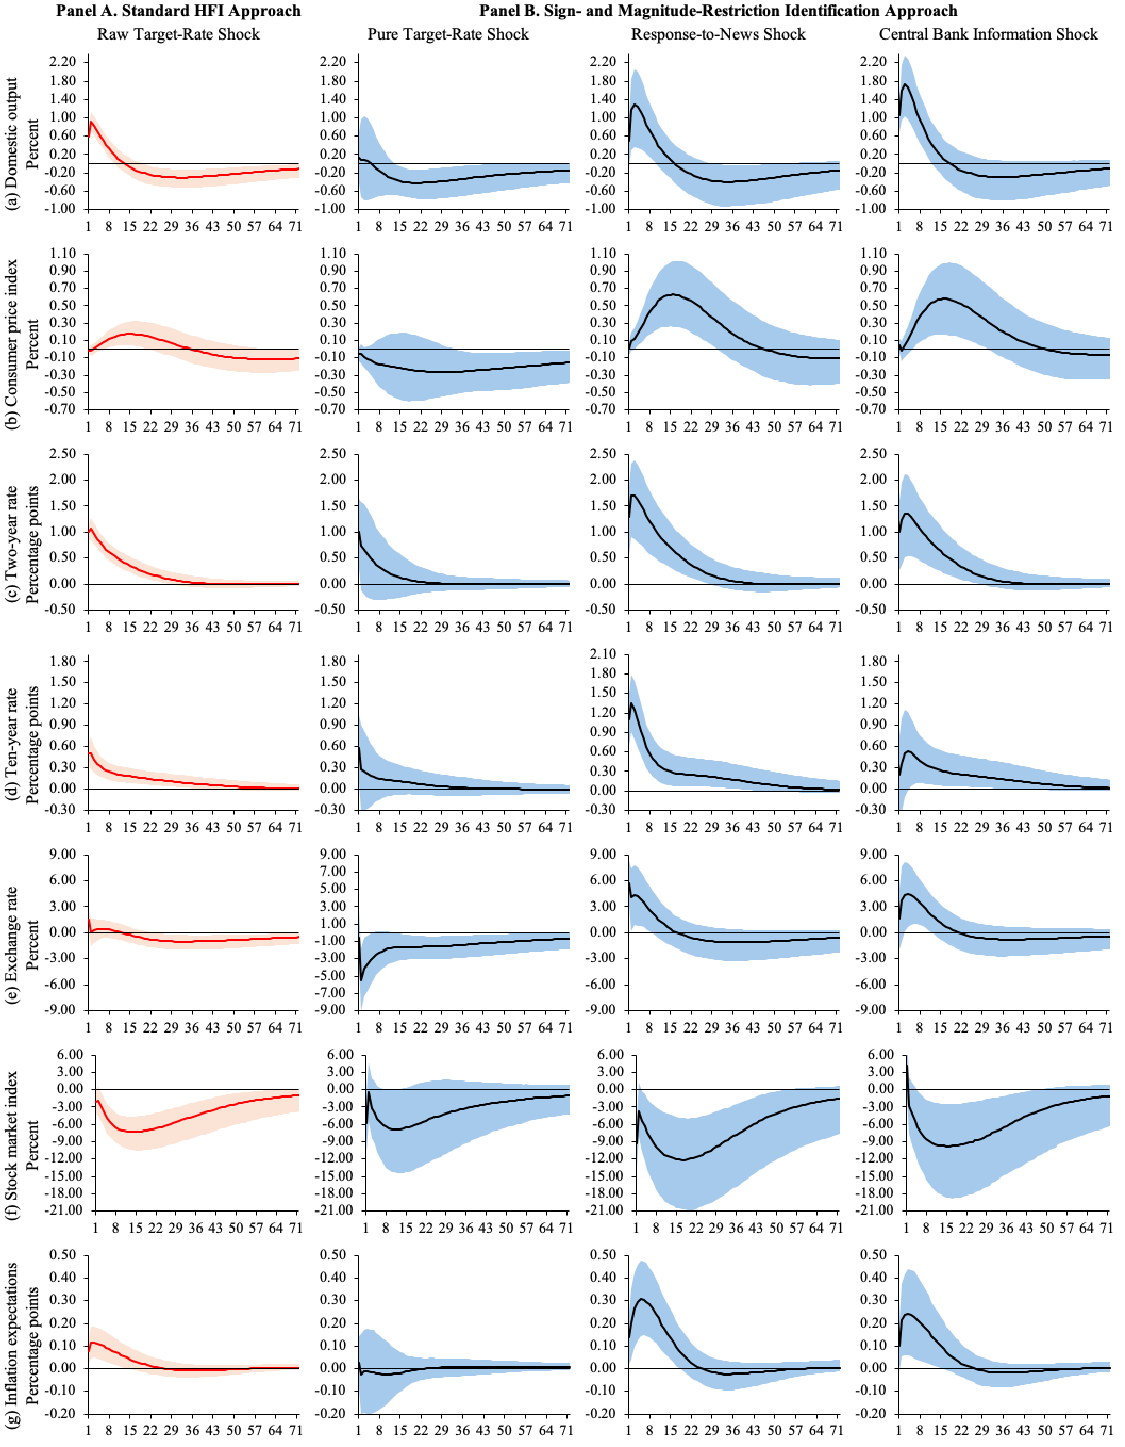
\includegraphics[width=\linewidth]{TR-2024m12_gs2.pdf}
}
\caption[5pt]{Impulse Responses to Target-Rate, Response-to-News, and Central Bank Information Shocks: Specification including the Two-Year Government Bond Yield instead of the One-Year Government Bond Yield}
\end{center}
\begin{footnotesize} 
Notes: Responses  are  presented  for a 72-month horizon with the associated 68\% highest posterior density intervals (HPDIs).
\end{footnotesize} 
\end{figure}

\renewcommand{\thefigure}{\thesection{}.1}
\begin{figure}[htbp]
\hypertarget{Figure 2}{}
\hypertarget{Panel AF2}{}
\hypertarget{Panel BF2}{}
\begin{center}
\resizebox{14cm}{!} {

\includegraphics[width=\linewidth]{FG-2024m12_gs2.pdf}
}
\caption[5pt]{Impulse Responses to Forward Guidance, Response-to-News, and Central Bank Information Shocks: Specification including the Two-Year Government Bond Yield instead of the One-Year Government Bond Yield}
\end{center}
\begin{footnotesize} 
Notes: Responses  are  presented  for a 72-month horizon with the associated 68\% highest posterior density intervals (HPDIs).
\end{footnotesize} 
\end{figure}

\renewcommand{\thefigure}{\thesection{}.1}
\begin{figure}[htbp]
\hypertarget{Figure 2}{}
\hypertarget{Panel AF2}{}
\hypertarget{Panel BF2}{}
\begin{center}
\resizebox{12cm}{!} {
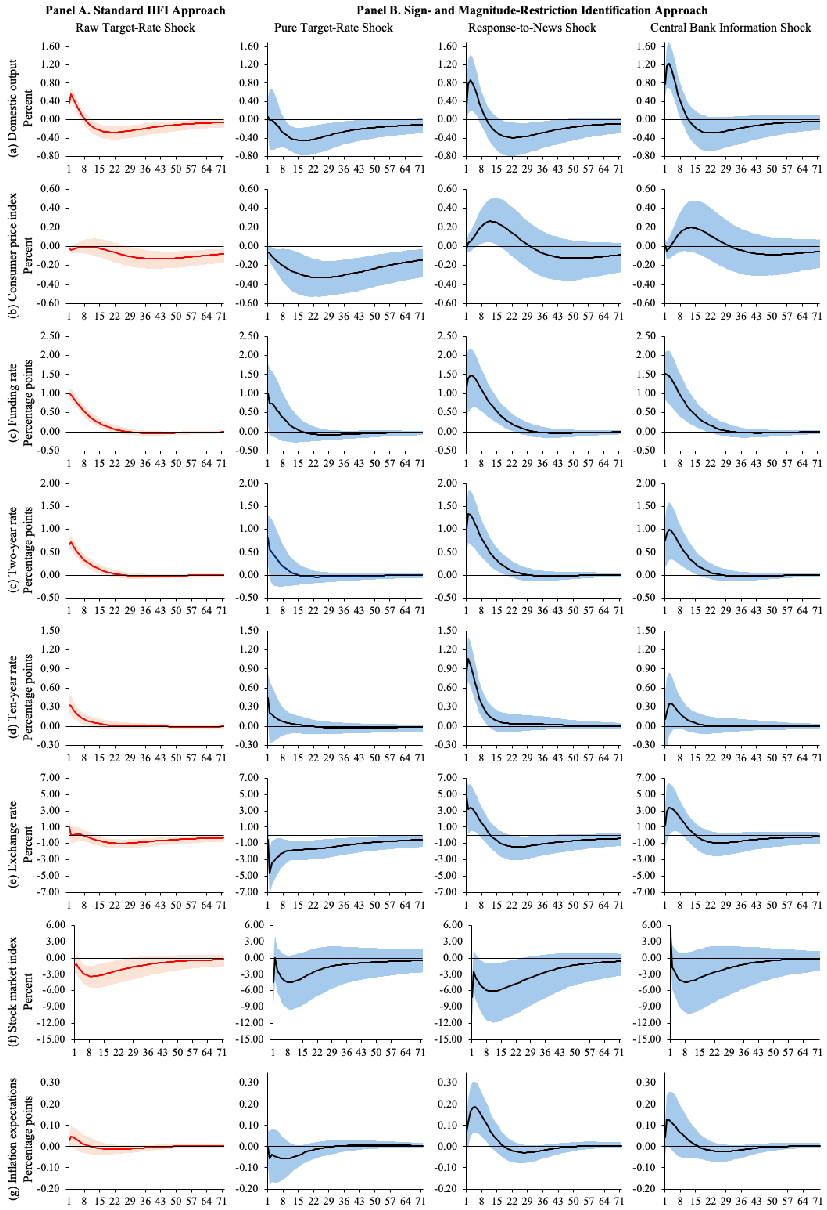
\includegraphics[width=\linewidth]{TR-2024m12_Fund_and_gs2.pdf}
}
\caption[5pt]{Impulse Responses to Target-Rate, Response-to-News, and Central Bank Information Shocks: Specification including the Interbank Funding Interest Rate and the Two-Year Government Bond Yield}
\end{center}
\begin{footnotesize} 
Notes: Responses  are  presented  for a 72-month horizon with the associated 68\% highest posterior density intervals (HPDIs).
\end{footnotesize} 
\end{figure}

\renewcommand{\thefigure}{\thesection{}.1}
\begin{figure}[htbp]
\hypertarget{Figure 2}{}
\hypertarget{Panel AF2}{}
\hypertarget{Panel BF2}{}
\begin{center}
\resizebox{12cm}{!} {

\includegraphics[width=\linewidth]{FG-2024m12_Fund_and_gs2.pdf}
}
\caption[5pt]{Impulse Responses to Forward Guidance, Response-to-News, and Central Bank Information Shocks: Specification including the Interbank Funding Interest Rate and the Two-Year Government Bond Yield}
\end{center}
\begin{footnotesize} 
Notes: Responses  are  presented  for a 72-month horizon with the associated 68\% highest posterior density intervals (HPDIs).
\end{footnotesize} 
\end{figure}

\renewcommand{\thefigure}{\thesection{}.1}
\begin{figure}[htbp]
\hypertarget{Figure 2}{}
\hypertarget{Panel AF2}{}
\hypertarget{Panel BF2}{}
\begin{center}
\resizebox{14cm}{!} {
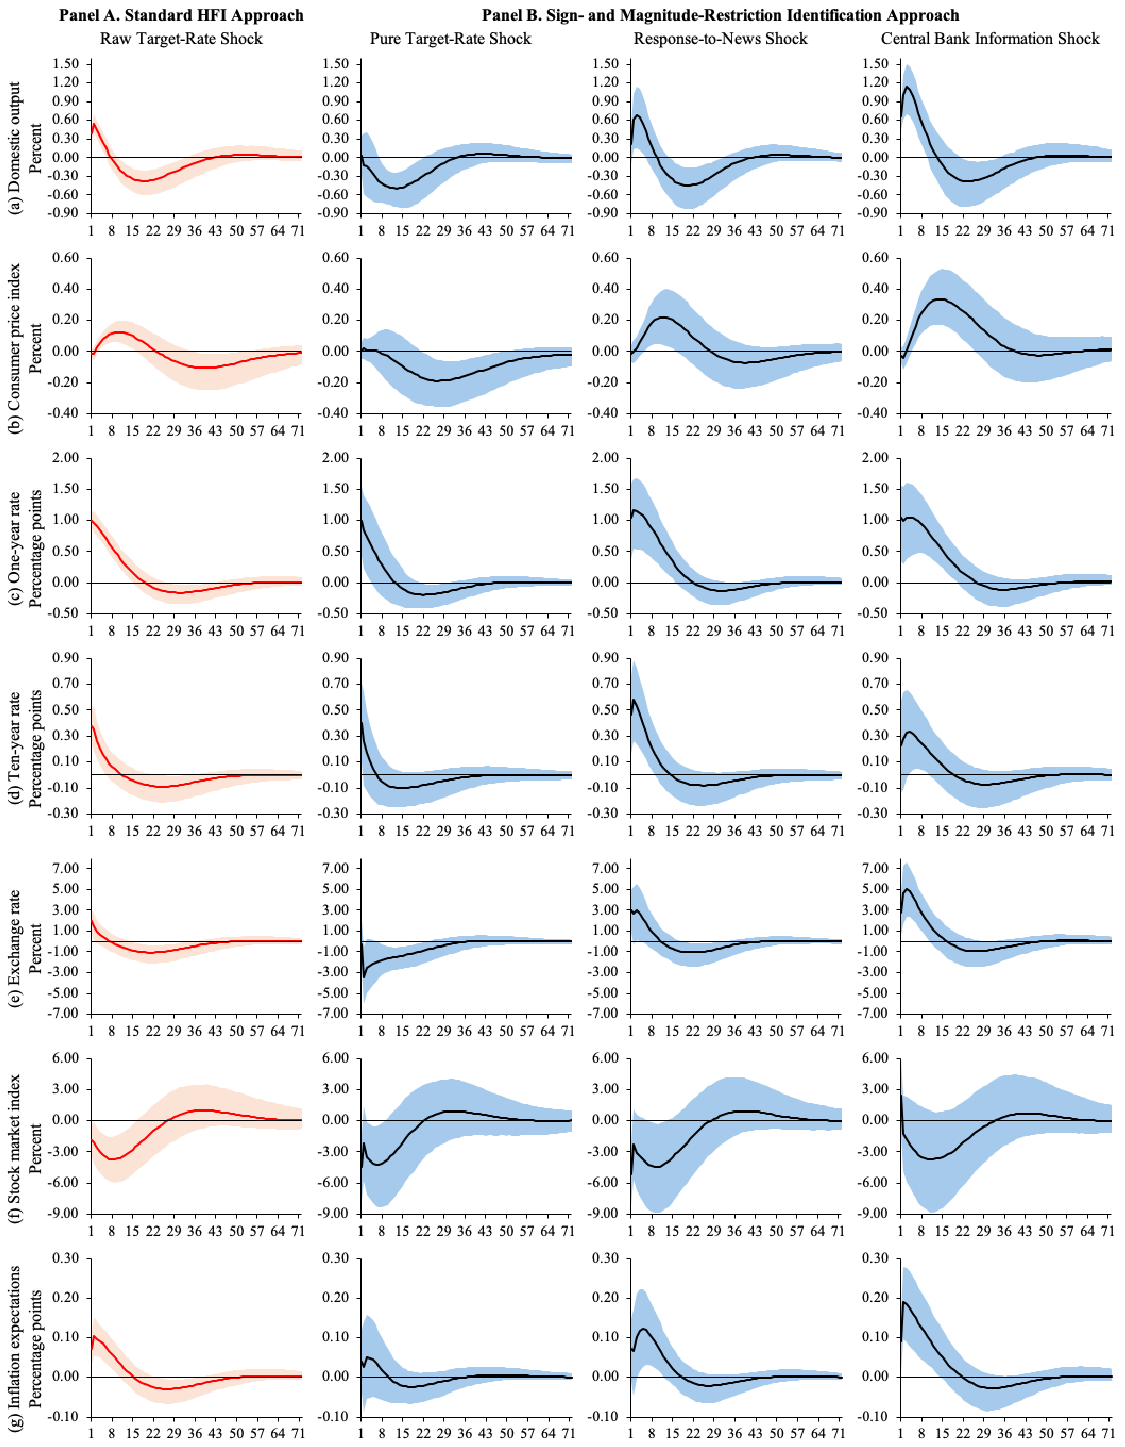
\includegraphics[width=\linewidth]{TR-2019.pdf}
}
\caption[5pt]{Impulse Responses to Target-Rate, Response-to-News, and Central Bank Information Shocks: Sample 2002-2019}
\end{center}
\begin{footnotesize} 
Notes: Responses  are  presented  for a 72-month horizon with the associated 68\% highest posterior density intervals (HPDIs).
\end{footnotesize} 
\end{figure}

\renewcommand{\thefigure}{\thesection{}.1}
\begin{figure}[htbp]
\hypertarget{Figure 2}{}
\hypertarget{Panel AF2}{}
\hypertarget{Panel BF2}{}
\begin{center}
\resizebox{14cm}{!} {

\includegraphics[width=\linewidth]{FG-2019m12.pdf}
}
\caption[5pt]{Impulse Responses to Forward Guidance, Response-to-News, and Central Bank Information Shocks: Sample 2002-2019}
\end{center}
\begin{footnotesize} 
Notes: Responses  are  presented  for a 72-month horizon with the associated 68\% highest posterior density intervals (HPDIs).
\end{footnotesize} 
\end{figure}

\renewcommand{\thefigure}{\thesection{}.1}
\begin{figure}[htbp]
\hypertarget{Figure 2}{}
\hypertarget{Panel AF2}{}
\hypertarget{Panel BF2}{}
\begin{center}
\resizebox{14cm}{!} {
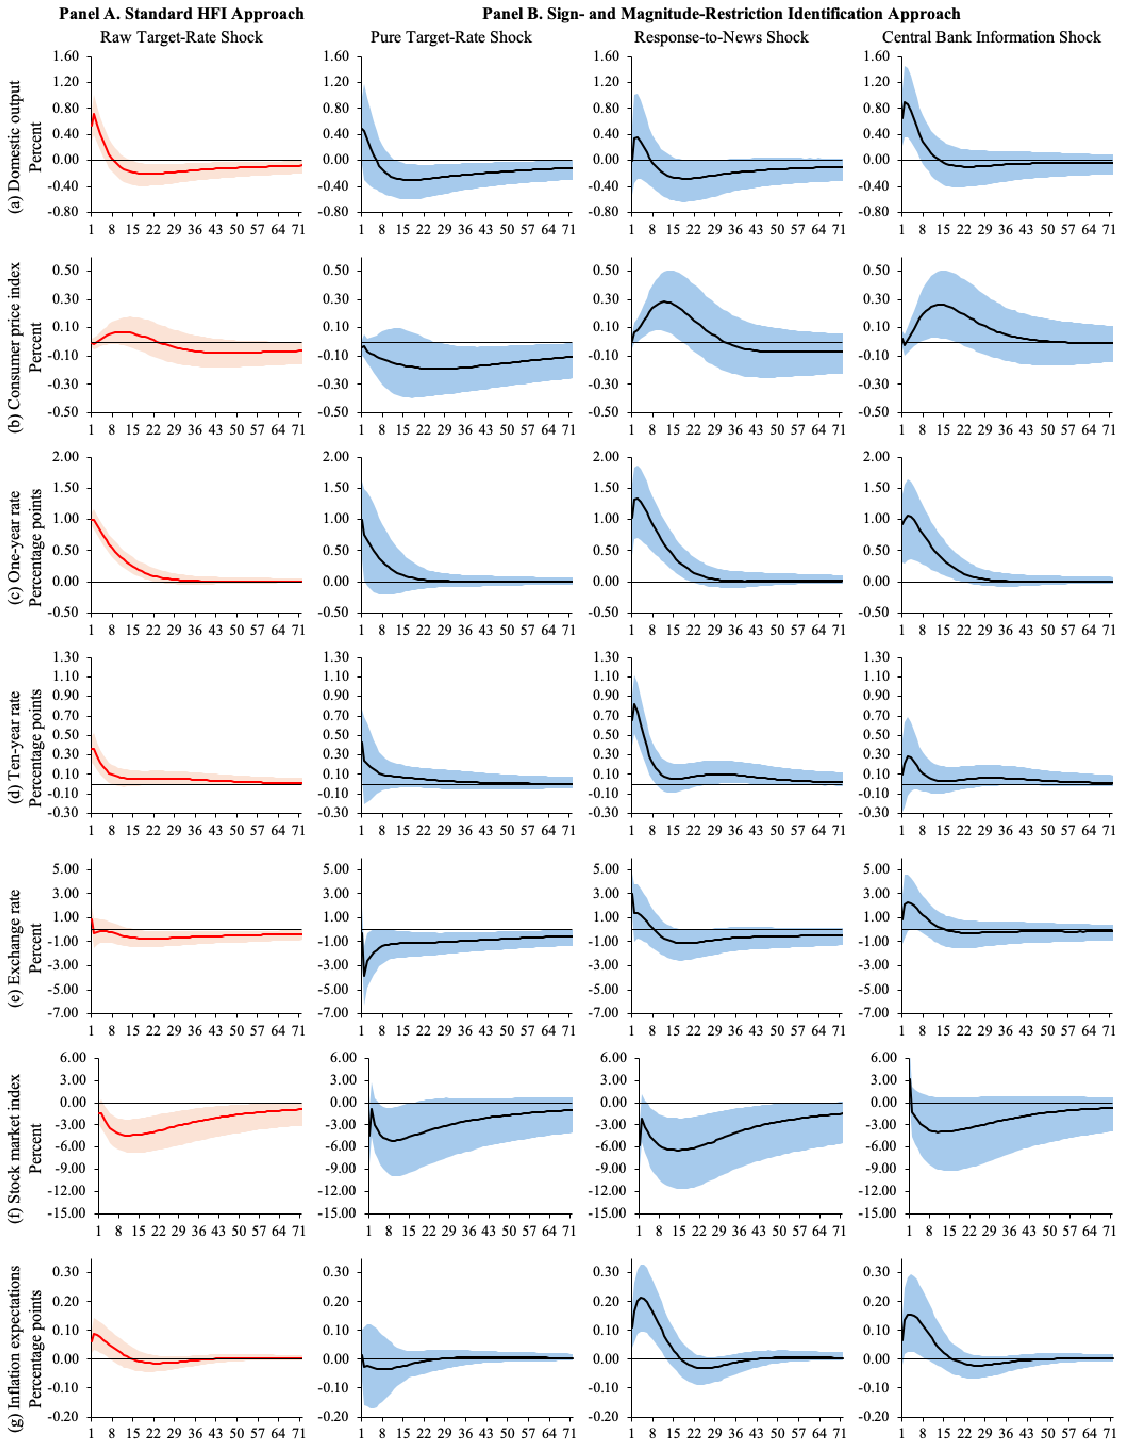
\includegraphics[width=\linewidth]{TR_igae.pdf}
}
\caption[5pt]{Impulse Responses to Target-Rate, Response-to-News, and Central Bank Information Shocks: Specification including IGAE instead of Interpolated GDP}
\end{center}
\begin{footnotesize} 
Notes: Responses  are  presented  for a 72-month horizon with the associated 68\% highest posterior density intervals (HPDIs).
\end{footnotesize} 
\end{figure}

\renewcommand{\thefigure}{\thesection{}.1}
\begin{figure}[htbp]
\hypertarget{Figure 2}{}
\hypertarget{Panel AF2}{}
\hypertarget{Panel BF2}{}
\begin{center}
\resizebox{14cm}{!} {

\includegraphics[width=\linewidth]{FG-igae.pdf}
}
\caption[5pt]{Impulse Responses to Forward Guidance, Response-to-News, and Central Bank Information Shocks: Specification including IGAE instead of Interpolated GDP}
\end{center}
\begin{footnotesize} 
Notes: Responses  are  presented  for a 72-month horizon with the associated 68\% highest posterior density intervals (HPDIs).
\end{footnotesize} 
\end{figure}

\renewcommand{\thefigure}{\thesection{}.1}
\begin{figure}[htbp]
\hypertarget{Figure 2}{}
\hypertarget{Panel AF2}{}
\hypertarget{Panel BF2}{}
\begin{center}
\resizebox{14cm}{!} {
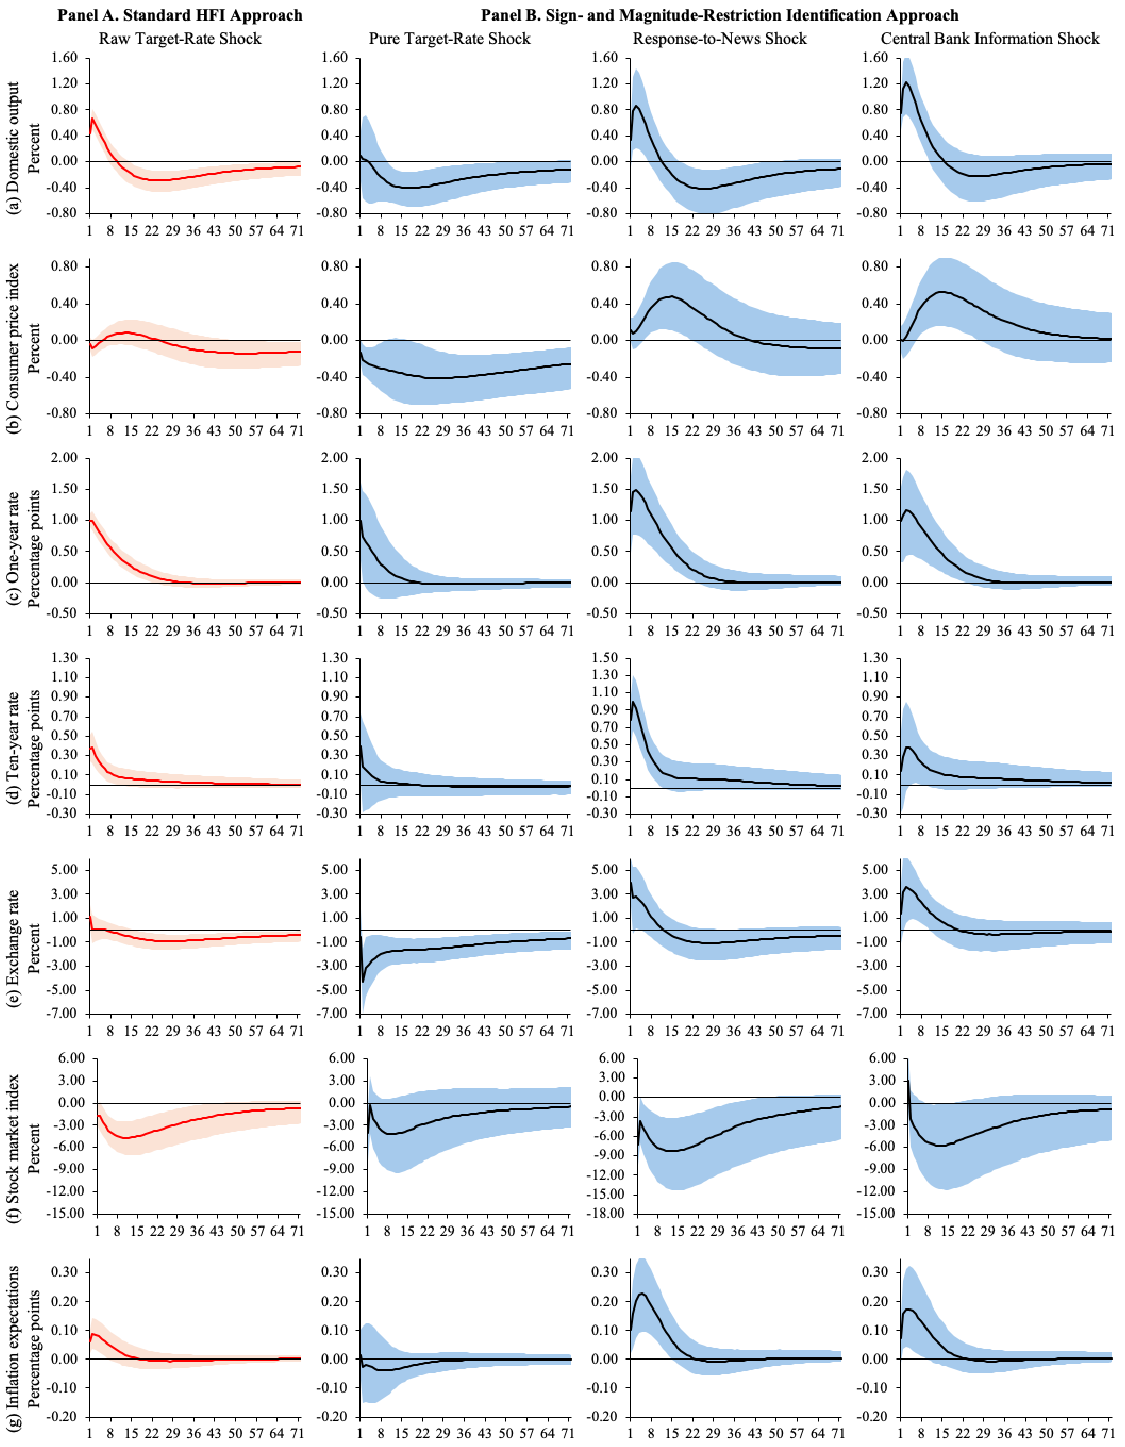
\includegraphics[width=\linewidth]{TR_inpc.pdf}
}
\caption[5pt]{Impulse Responses to Target-Rate, Response-to-News, and Central Bank Information Shocks: Specification including Headline INPC instead of Core INPC}
\end{center}
\begin{footnotesize} 
Notes: Responses  are  presented  for a 72-month horizon with the associated 68\% highest posterior density intervals (HPDIs).
\end{footnotesize} 
\end{figure}

\renewcommand{\thefigure}{\thesection{}.1}
\begin{figure}[htbp]
\hypertarget{Figure 2}{}
\hypertarget{Panel AF2}{}
\hypertarget{Panel BF2}{}
\begin{center}
\resizebox{14cm}{!} {

\includegraphics[width=\linewidth]{FG-inpc.pdf}
}
\caption[5pt]{Impulse Responses to Forward Guidance, Response-to-News, and Central Bank Information Shocks: Specification including Headline INPC instead of Core INPC}
\end{center}
\begin{footnotesize} 
Notes: Responses  are  presented  for a 72-month horizon with the associated 68\% highest posterior density intervals (HPDIs).
\end{footnotesize} 
\end{figure}

\begin{table}[htbp]
\centering
\caption{Projection of High-Frequency Monetary Policy Surprises: Extended vs.\ Baseline Specification}
\resizebox{0.65\textwidth}{!}{
\begin{tabular}{lcccc}
\toprule
 & \multicolumn{2}{c}{Target-rate surprise} & \multicolumn{2}{c}{FG surprise} \\
\cmidrule(lr){2-3} \cmidrule(lr){4-5}
 & Extended & Baseline & Extended & Baseline \\
\midrule

\multicolumn{5}{l}{\textbf{\emph{Domestic news}}} \\[0.2em]

$\Delta \log$ domestic output (6m)
& -0.037 & -0.036 
& 0.139 & 0.239 \\
& (0.193) & (0.177)
& (0.726) & (0.674) \\

$\Delta \log$ CPI (6m)
& -0.248 & -0.287 
& 1.985 & 2.109 \\
& (1.269) & (1.246)
& (3.289) & (3.483) \\

$\Delta \log$ Stock market index (3m)
& 0.036 & -- 
& 0.122 & -- \\
& (0.093) & 
& (0.230) & \\

$\Delta \log$ MXN/USD (3m)
& -0.010 & 0.007 
& 1.124** & 0.962** \\
& (0.191) & (0.168)
& (0.442) & (0.410) \\

$\Delta$ FX implied volatility (3m)
& 0.004* & 0.004* 
& -0.009** & -0.010** \\
& (0.002) & (0.002)
& (0.004) & (0.004) \\

$\Delta$ Interbank rate (3m)
& 0.014 & 0.022 
& -0.003 & -0.010 \\
& (0.027) & (0.015)
& (0.057) & (0.027) \\

$\Delta$ 2-year gov. yield (3m)
& 0.020 & 0.030* 
& 0.114 & 0.008 \\
& (0.024) & (0.015)
& (0.075) & (0.039) \\

$\Delta$ 10-year gov. yield (3m)
& 0.023 & -- 
& -0.136 & -- \\
& (0.042) & 
& (0.114) & \\

$\Delta$ Yield curve slope (3m)
& -0.018 & -- 
& 0.055 & -- \\
& (0.043) & 
& (0.093) & \\[0.4em]

\multicolumn{5}{l}{\textbf{\emph{External news}}} \\[0.2em]

$\Delta \log$ Industrial prod. (6m)
& -0.006 & 0.007 
& 0.718 & 0.782 \\
& (0.296) & (0.261)
& (0.881) & (0.849) \\

$\Delta \log$ US CPI (6m)
& 1.143 & 1.201 
& -1.596 & -1.219 \\
& (0.916) & (0.979)
& (1.913) & (2.053) \\

$\Delta \log$ S\&P 500 (3m)
& 0.152 & 0.129 
& -0.056 & 0.252 \\
& (0.171) & (0.143)
& (0.396) & (0.337) \\

$\Delta \log$ VIX (3m)
& 0.011 & -- 
& -0.034 & -- \\
& (0.025) & 
& (0.070) & \\

$\Delta$ 2-year Treasury yield (3m)
& -0.001 & -0.007 
& 0.042 & 0.091** \\
& (0.030) & (0.021)
& (0.068) & (0.040) \\

$\Delta$ 10-year Treasury yield (3m)
& -0.064* & -0.052* 
& 0.005 & -0.095* \\
& (0.038) & (0.026)
& (0.100) & (0.054) \\

$\Delta$ Yield curve slope (3m)
& 0.008 & -- 
& -0.030 & -- \\
& (0.023) & 
& (0.053) & \\

$\Delta \log$ Brent oil price (3m)
& 0.078* & 0.078* 
& 0.113 & 0.123 \\
& (0.044) & (0.045)
& (0.106) & (0.110) \\[0.4em]

\multicolumn{5}{l}{\textbf{\emph{Lagged monetary policy surprises}}} \\[0.2em]

Surprise$_{t-1}$
& 0.020 & 0.021 
& -0.276*** & -0.225** \\
& (0.123) & (0.120)
& (0.096) & (0.097) \\

Surprise$_{t-2}$
& -0.013 & -- 
& -0.120 & -- \\
& (0.087) & 
& (0.084) & \\

\midrule
$R^2$
& 0.227 & 0.224
& 0.195 & 0.154 \\

Adjusted $R^2$
& 0.151 & 0.173
& 0.115 & 0.099 \\

Observations
& 213 & 213
& 213 & 213 \\

\bottomrule
\end{tabular}}
\begin{flushleft}
\footnotesize
\parbox{0.97\textwidth}{
\textit{Notes}: The extended specification augments the baseline projection reported in Table~1 with a broader set of macro-financial controls used in the related literature. Variables not included in the baseline are denoted by ``--''. Standard errors (in parentheses) are heteroskedasticity- and autocorrelation-consistent (HAC), computed using a Newey--West estimator. $^{*}$, $^{**}$, and $^{***}$ denote significance at the 10\%, 5\%, and 1\% levels, respectively.
}
\end{flushleft}
\end{table}

\renewcommand{\thefigure}{\thesection{}.1}
\begin{figure}[htbp]
\hypertarget{Figure 2}{}
\hypertarget{Panel AF2}{}
\hypertarget{Panel BF2}{}
\begin{center}
\resizebox{11.5cm}{!} {
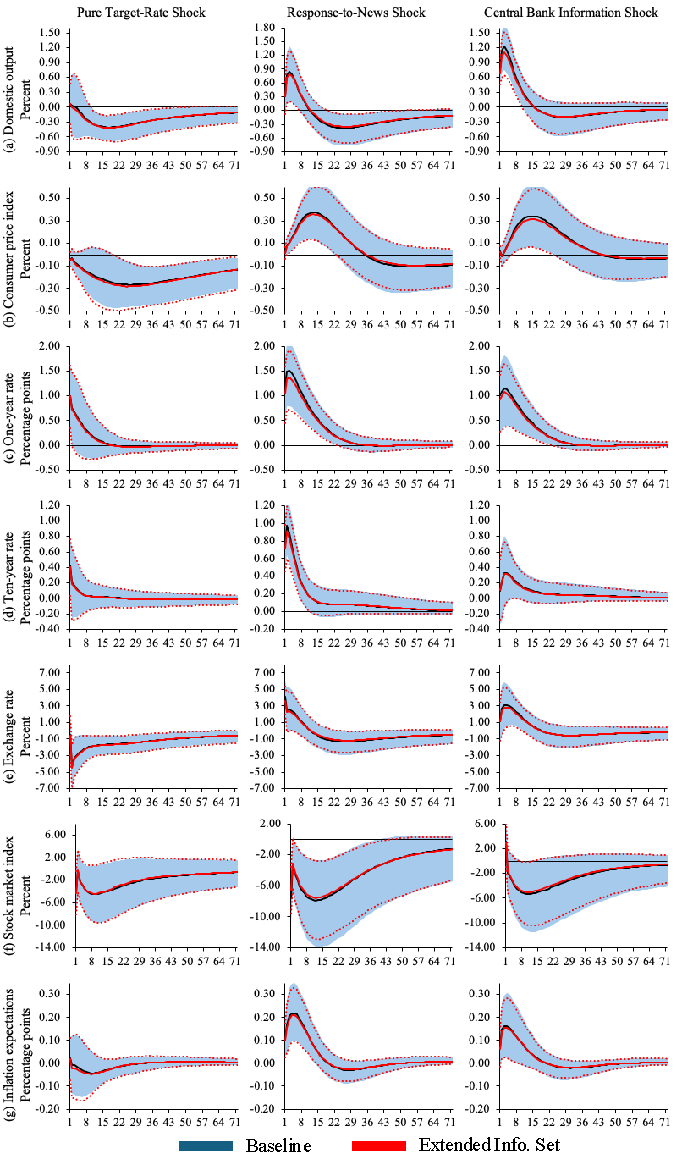
\includegraphics[width=\linewidth]{TR-Extended.pdf}
}
\caption[5pt]{Impulse Responses to Target-Rate, Response-to-News, and Central Bank Information Shocks: Baseline vs. Extended Information Set}
\end{center}
\begin{footnotesize} 
Notes: Responses  are  presented  for a 72-month horizon with the associated 68\% highest posterior density intervals (HPDIs).
\end{footnotesize} 
\end{figure}

\renewcommand{\thefigure}{\thesection{}.1}
\begin{figure}[htbp]
\hypertarget{Figure 2}{}
\hypertarget{Panel AF2}{}
\hypertarget{Panel BF2}{}
\begin{center}
\resizebox{11.5cm}{!} {
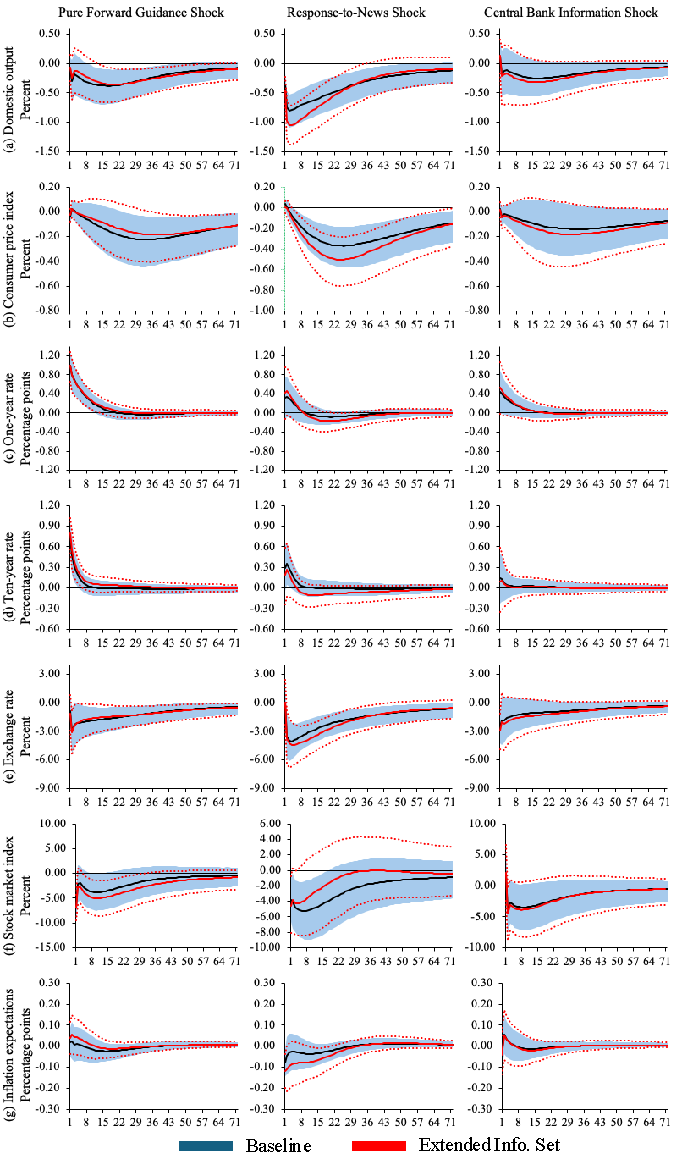
\includegraphics[width=\linewidth]{FG-Extended.pdf}
}
\caption[5pt]{Impulse Responses to Forward Guidance, Response-to-News, and Central Bank Information Shocks: Baseline vs. Extended Information Set}
\end{center}
\begin{footnotesize} 
Notes: Responses  are  presented  for a 72-month horizon with the associated 68\% highest posterior density intervals (HPDIs).
\end{footnotesize} 
\end{figure}



\begin{table}[htbp]
\centering
\caption{LASSO Selection over the Baseline Information Set}
\resizebox{0.85\textwidth}{!}{
\begin{tabular}{lcc}
\toprule
Variable (baseline set) & Target-rate surprise (LASSO) & FG surprise (LASSO) \\
\midrule
Constant & -0.883 & -1.406 \\

\multicolumn{3}{l}{\textbf{\emph{Domestic news}}} \\[0.2em]
$\Delta \log$ domestic output (6m) & -- & -- \\
$\Delta \log$ CPI (6m) & -- & -- \\
$\Delta \log$ MXN/USD (3m) & -- & -- \\
$\Delta$ FX implied volatility (3m) & 0.001 & -0.004 \\
$\Delta$ Interbank rate (3m) & 0.020 & -- \\
$\Delta$ 2-year gov. yield (3m) & 0.013 & -- \\[0.4em]

\multicolumn{3}{l}{\textbf{\emph{External news}}} \\[0.2em]
$\Delta \log$ Industrial prod. (6m) & 0.020 & -- \\
$\Delta \log$ US CPI (6m) & 0.849 & -- \\
$\Delta \log$ S\&P 500 (3m) & -- & -- \\
$\Delta$ 2-year Treasury yield (3m) & -0.002 & -- \\
$\Delta$ 10-year Treasury yield (3m) & -0.009 & -- \\
$\Delta \log$ Brent oil price (3m) & 0.003 & -- \\[0.4em]

\multicolumn{3}{l}{\textbf{\emph{Lagged monetary policy surprises}}} \\[0.2em]
Surprise$_{t-1}$ & 0.005 & -0.038 \\

\midrule
Optimal $\lambda$ & 0.798 & 2.729 \\
Non-zero coefficients & 10 & 3 \\
$R^2$ & 0.162 & 0.056 \\
Observations & 213 & 213 \\
\bottomrule
\end{tabular}}
\begin{flushleft}
\footnotesize
\parbox{0.95\textwidth}{
\textit{Notes}: The table reports LASSO (L1-penalized) projections estimated over the baseline information set used in Table~1, evaluated at the cross-validated optimal penalty parameter $\lambda$. Regressors are standardized prior to estimation. Variables not selected by the regularization procedure are denoted by ``--''.
}
\end{flushleft}
\end{table}


\renewcommand{\thefigure}{\thesection{}.1}
\begin{figure}[htbp]
\hypertarget{Figure 2}{}
\hypertarget{Panel AF2}{}
\hypertarget{Panel BF2}{}
\begin{center}
\resizebox{11.5cm}{!} {
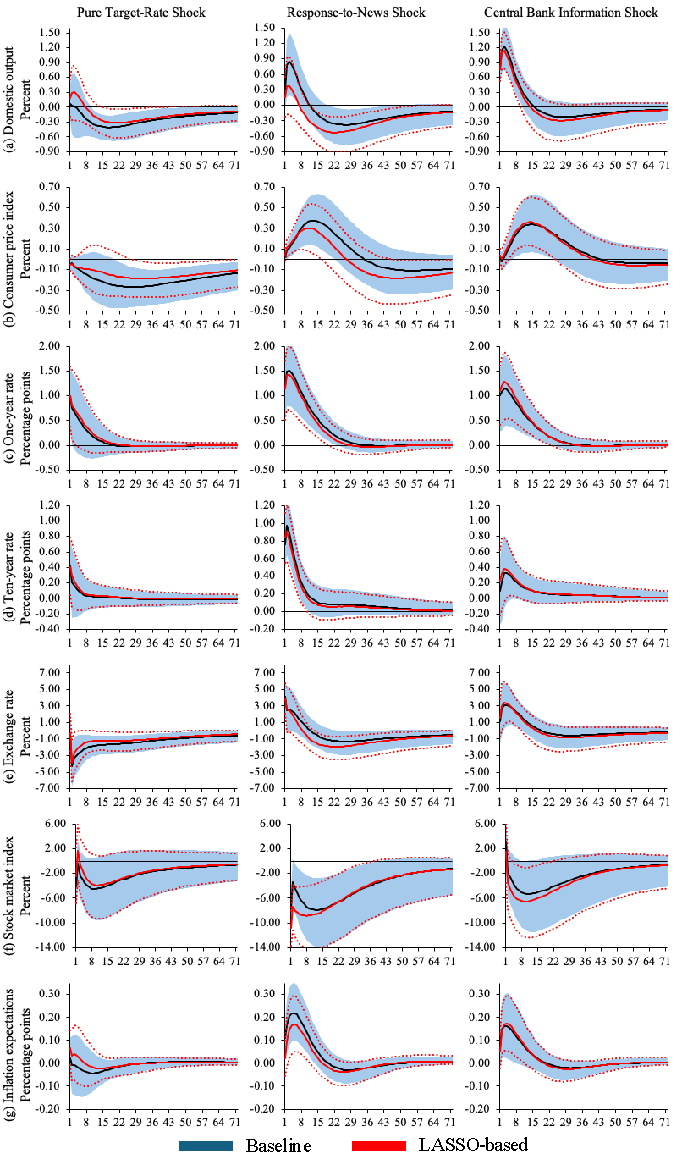
\includegraphics[width=\linewidth]{TR-Lasso.pdf}
}
\caption[5pt]{Impulse Responses to Target-Rate, Response-to-News, and Central Bank Information Shocks: Baseline vs. LASSO Diagnostic Projections}
\end{center}
\begin{footnotesize} 
Notes: Responses  are  presented  for a 72-month horizon with the associated 68\% highest posterior density intervals (HPDIs).
\end{footnotesize} 
\end{figure}

\renewcommand{\thefigure}{\thesection{}.1}
\begin{figure}[htbp]
\hypertarget{Figure 2}{}
\hypertarget{Panel AF2}{}
\hypertarget{Panel BF2}{}
\begin{center}
\resizebox{11.5cm}{!} {
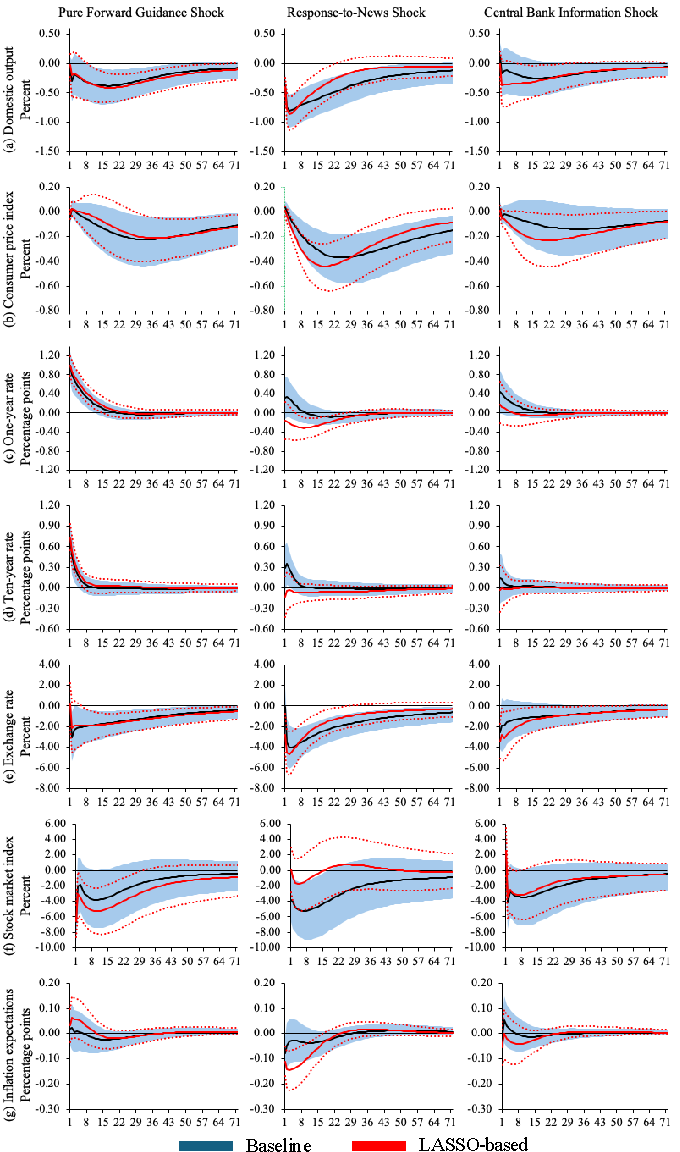
\includegraphics[width=\linewidth]{FG-Lasso.pdf}
}
\caption[5pt]{Impulse Responses to Forward Guidance, Response-to-News, and Central Bank Information Shocks: Baseline vs. LASSO Diagnostic Projections}
\end{center}
\begin{footnotesize} 
Notes: Responses  are  presented  for a 72-month horizon with the associated 68\% highest posterior density intervals (HPDIs).
\end{footnotesize} 
\end{figure}



\end{document}


